	\begin{figure}
			\centering
			\subfloat[SHREK]{
				\scalebox{.4}{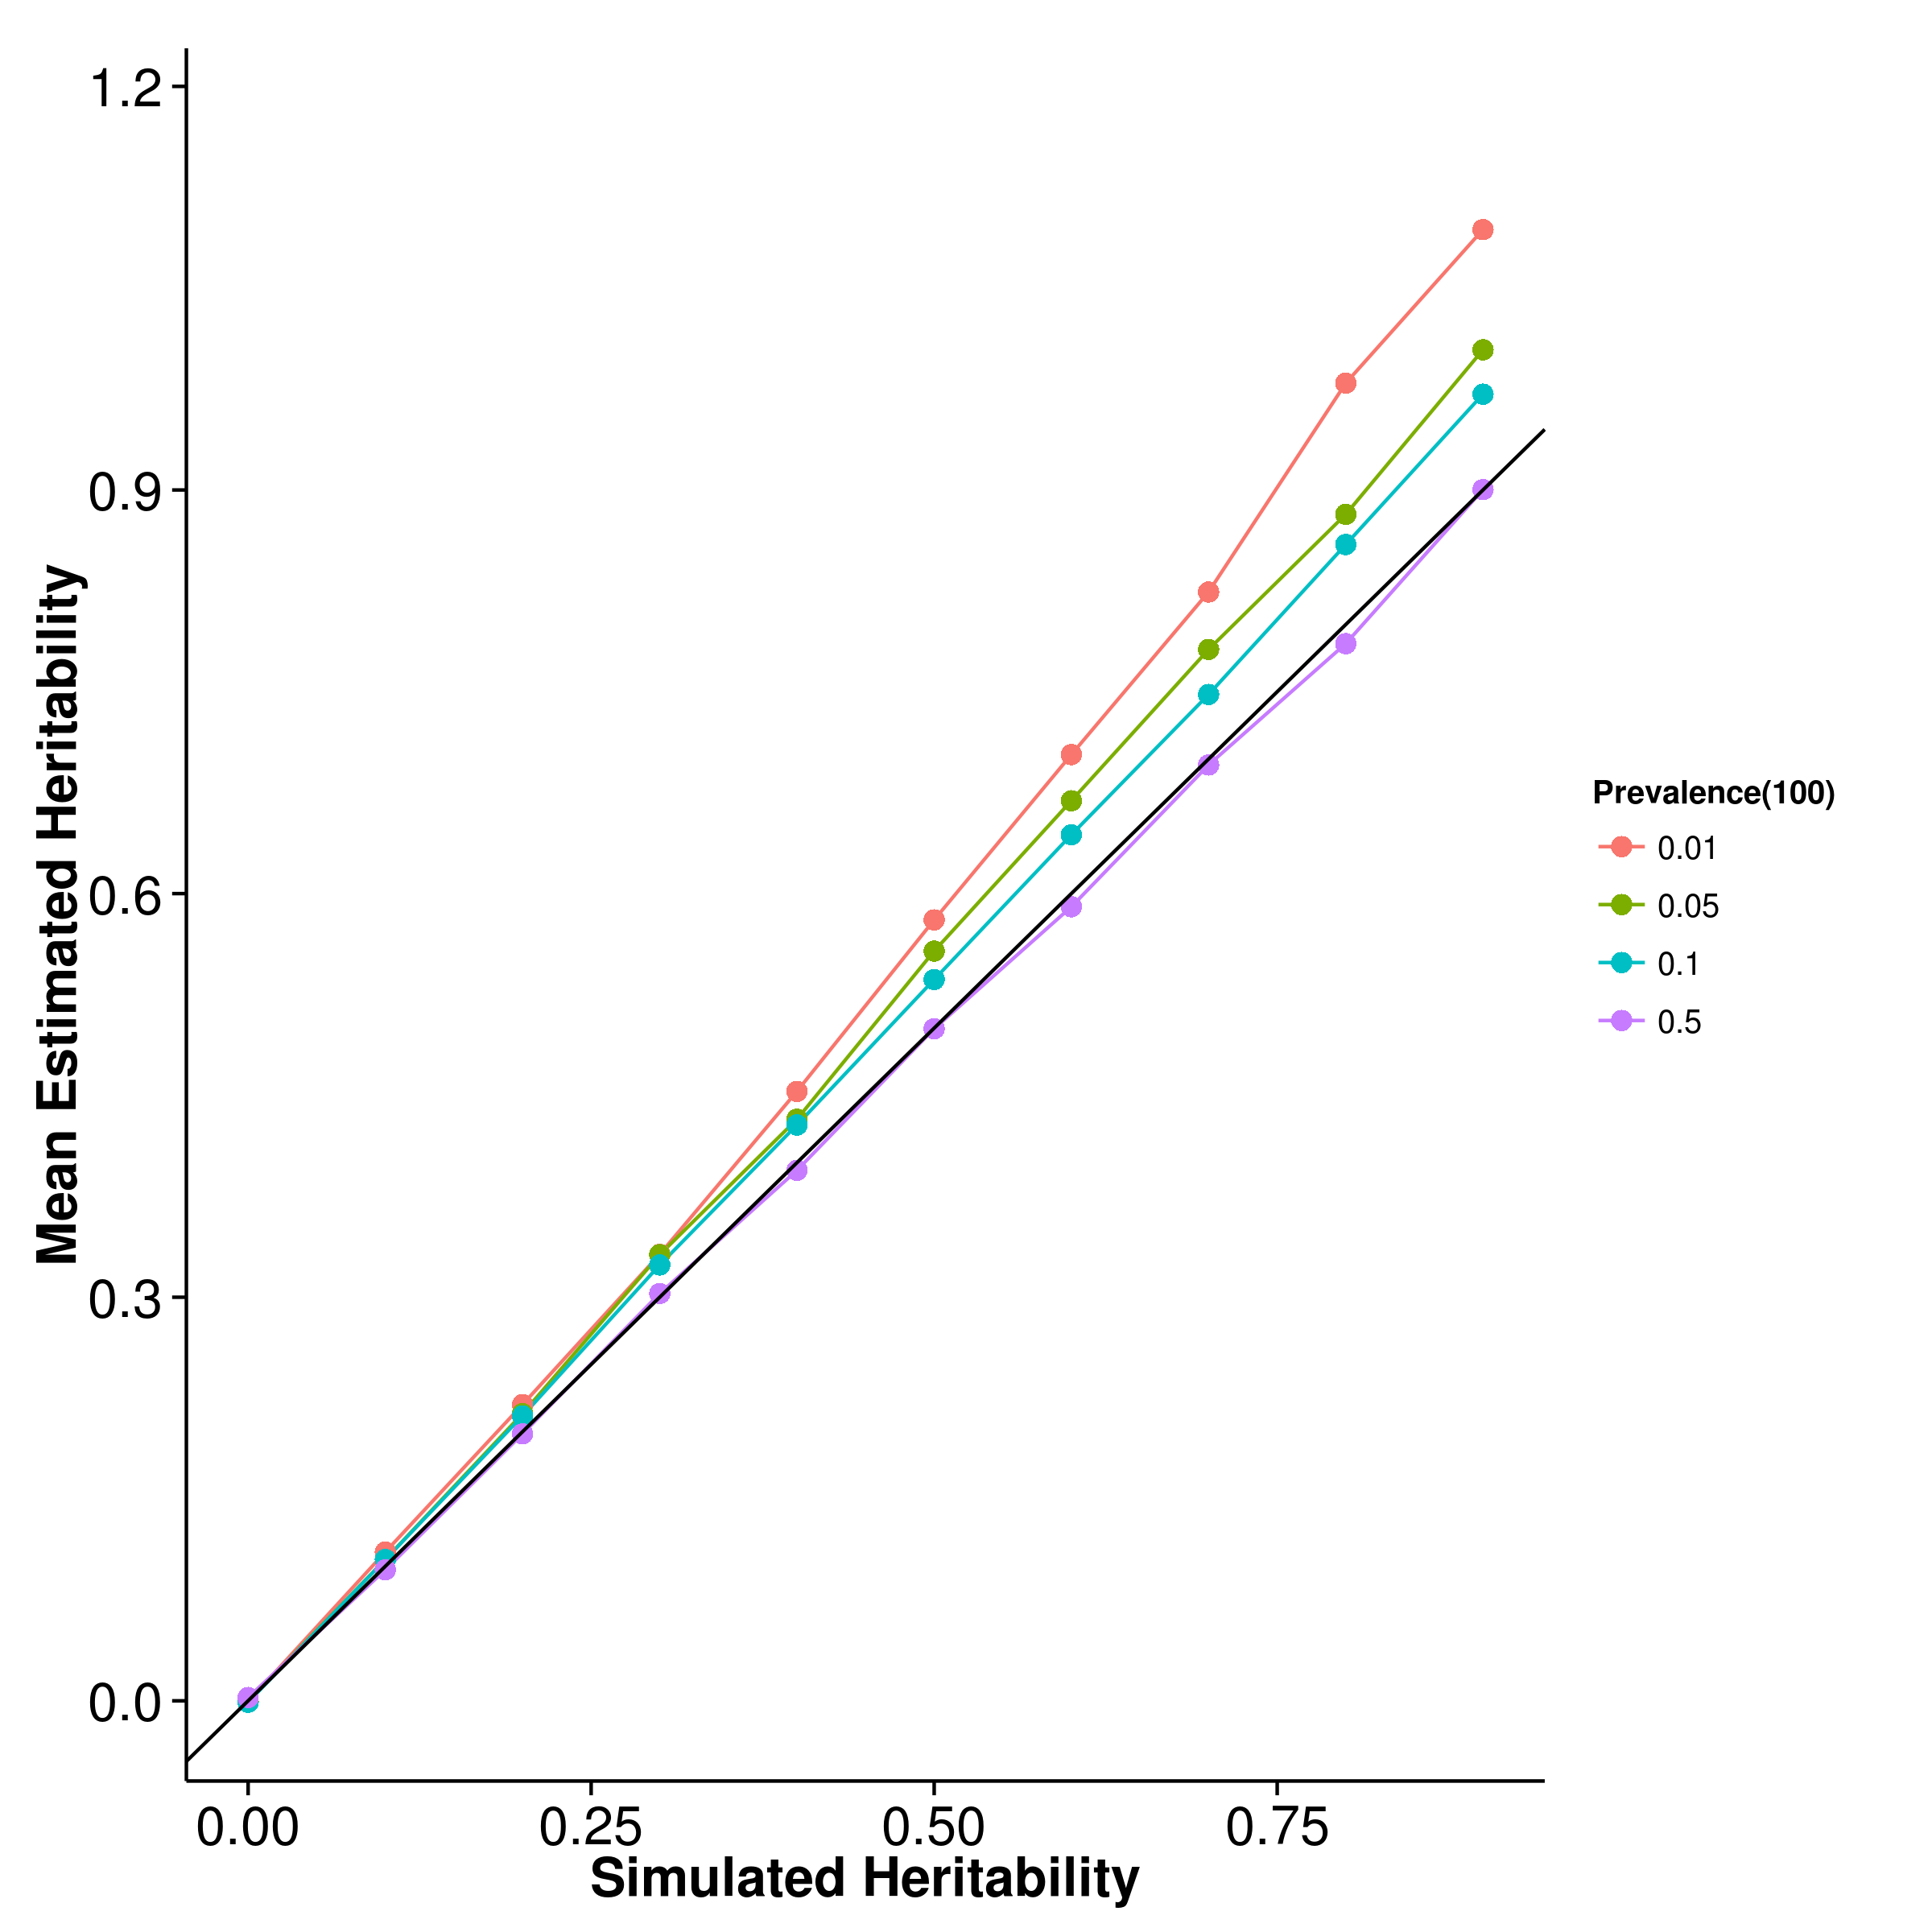
\includegraphics{figure/he_summary/cc_100c/shrek_CC_Rand_mean.png}}
				\label{fig:shrekCCRandMean}
			}
			\subfloat[GCTA]{
				\scalebox{.4}{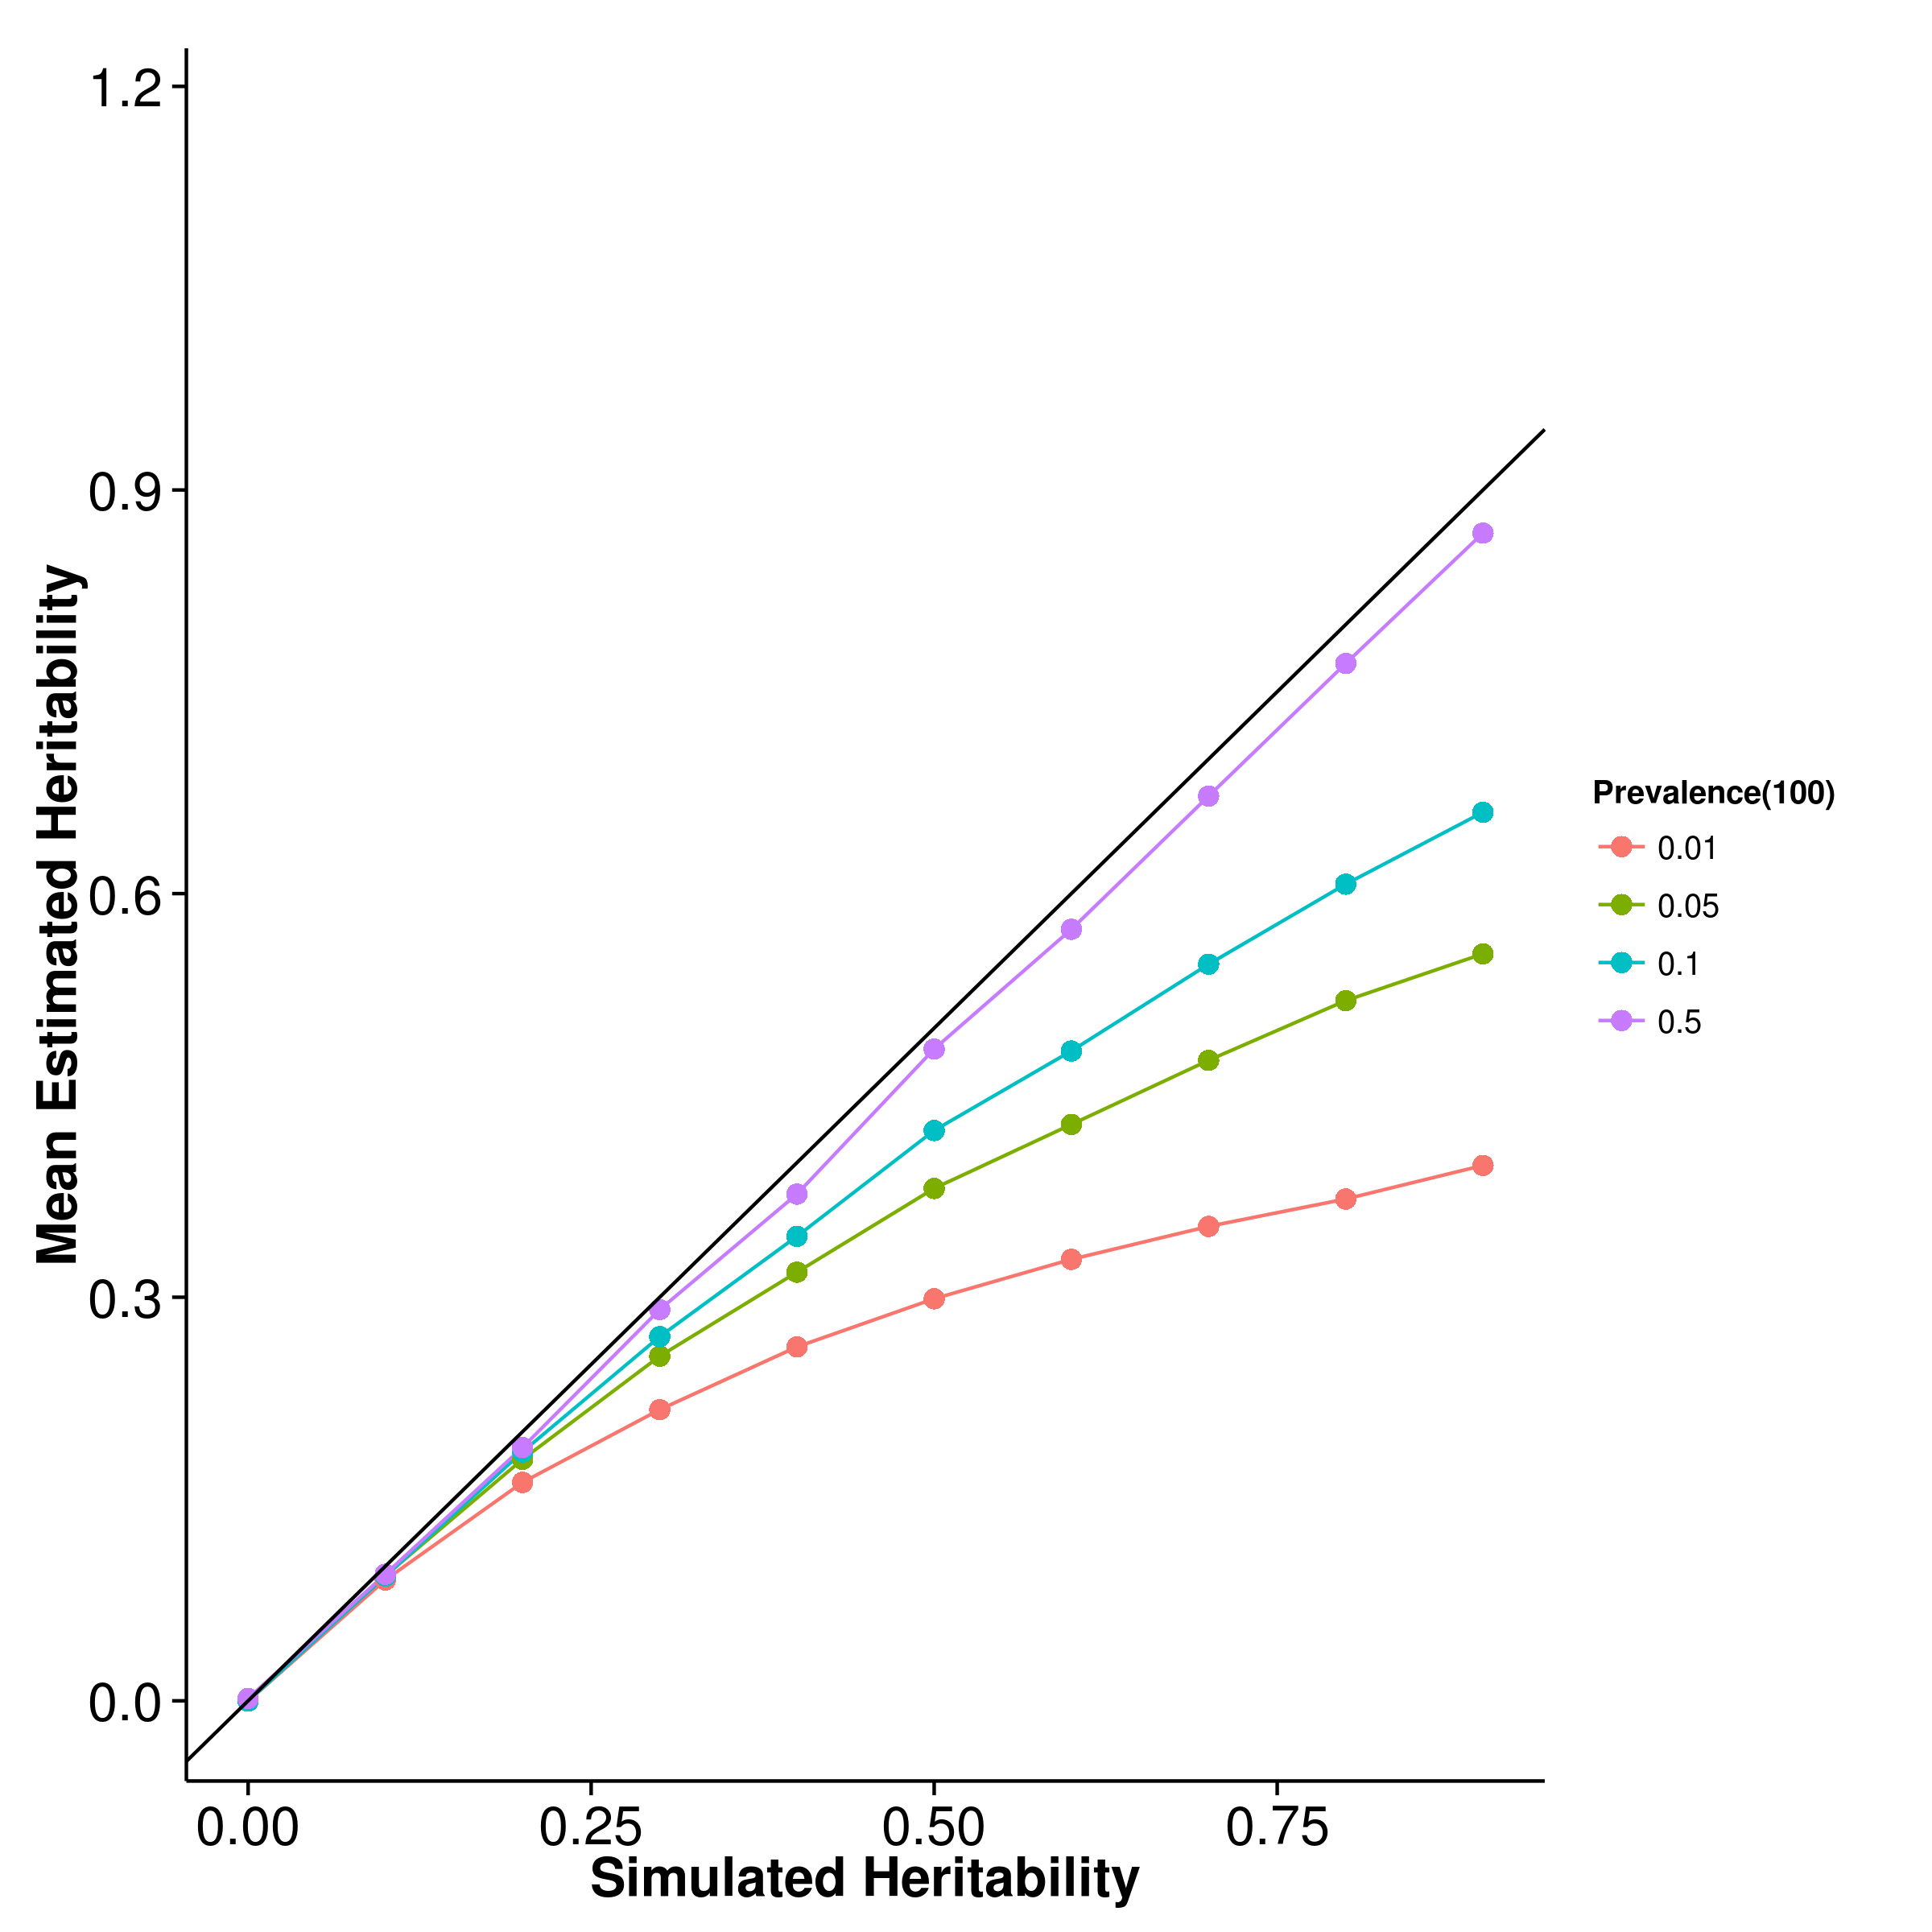
\includegraphics{figure/he_summary/cc_100c/gcta_CC_Rand_mean.png}}
				\label{fig:gctaCCRandMean}
			}\\
			\subfloat[LDSC with fix intercept]{
				\scalebox{.4}{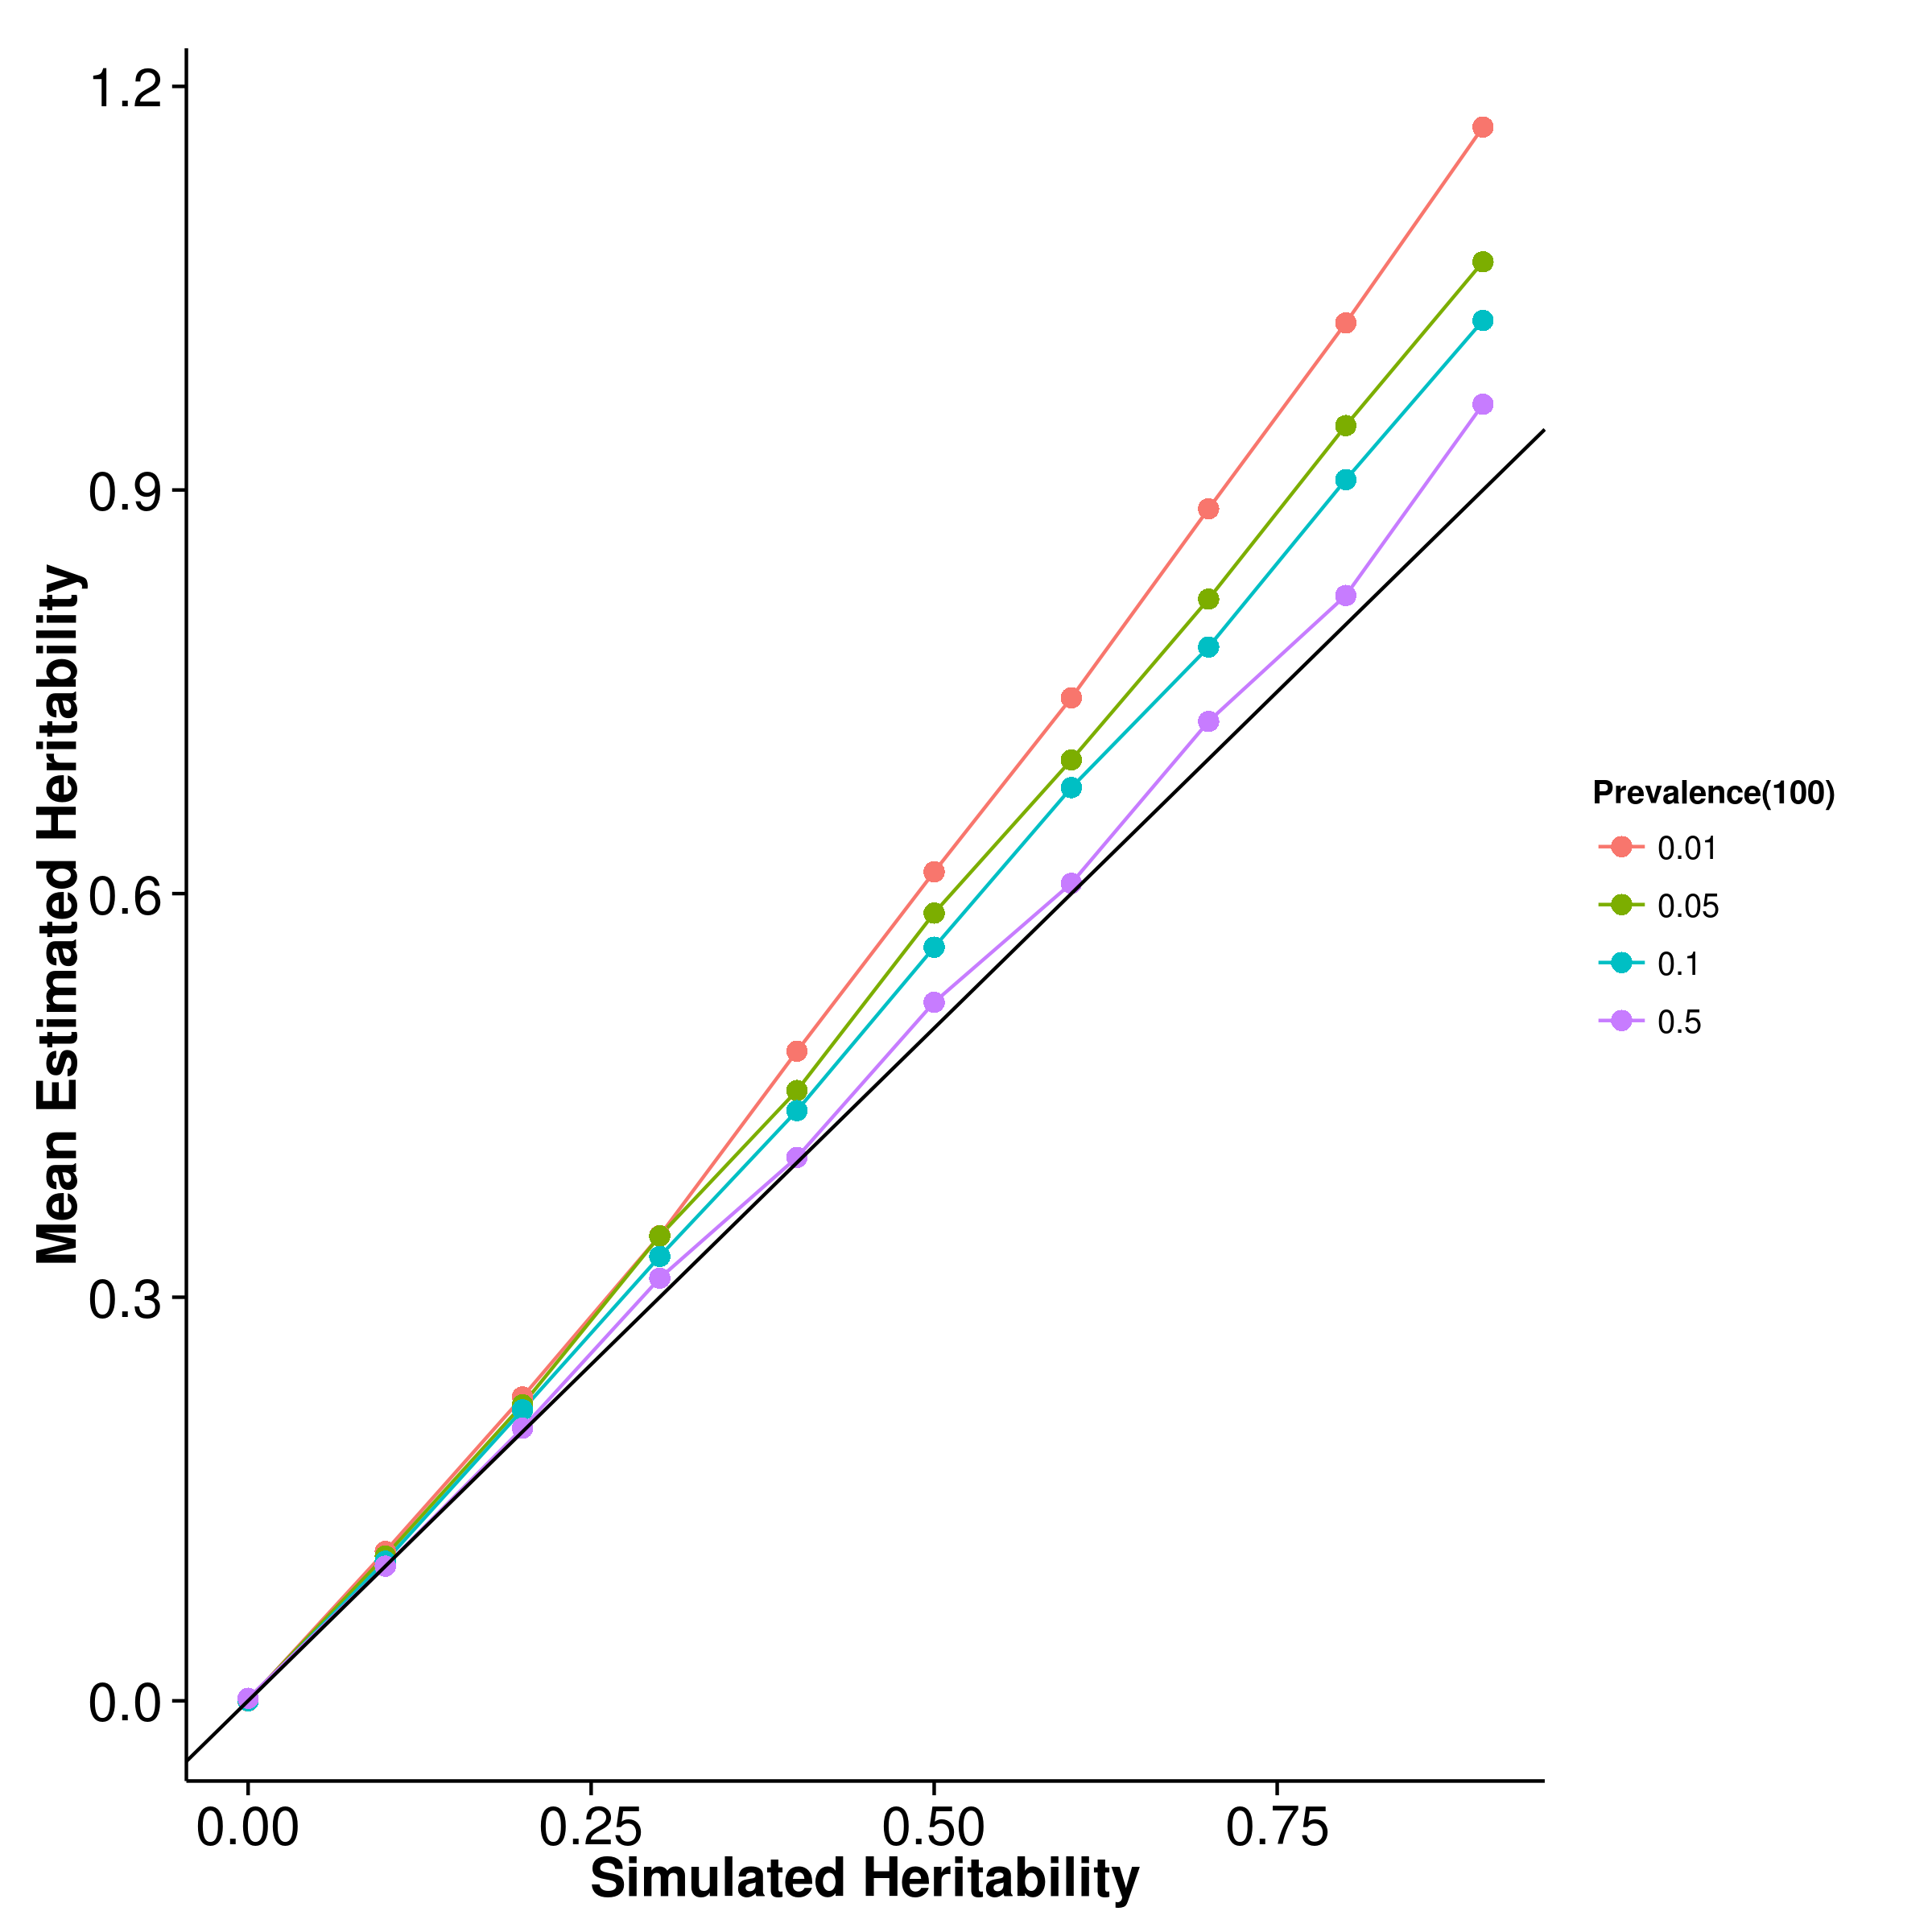
\includegraphics{figure/he_summary/cc_100c/ldsc_CC_Rand_mean.png}}
				\label{fig:ldscCCRandMean}
			}
			\subfloat[LDSC with intercept estimation]{
				
				\scalebox{.4}{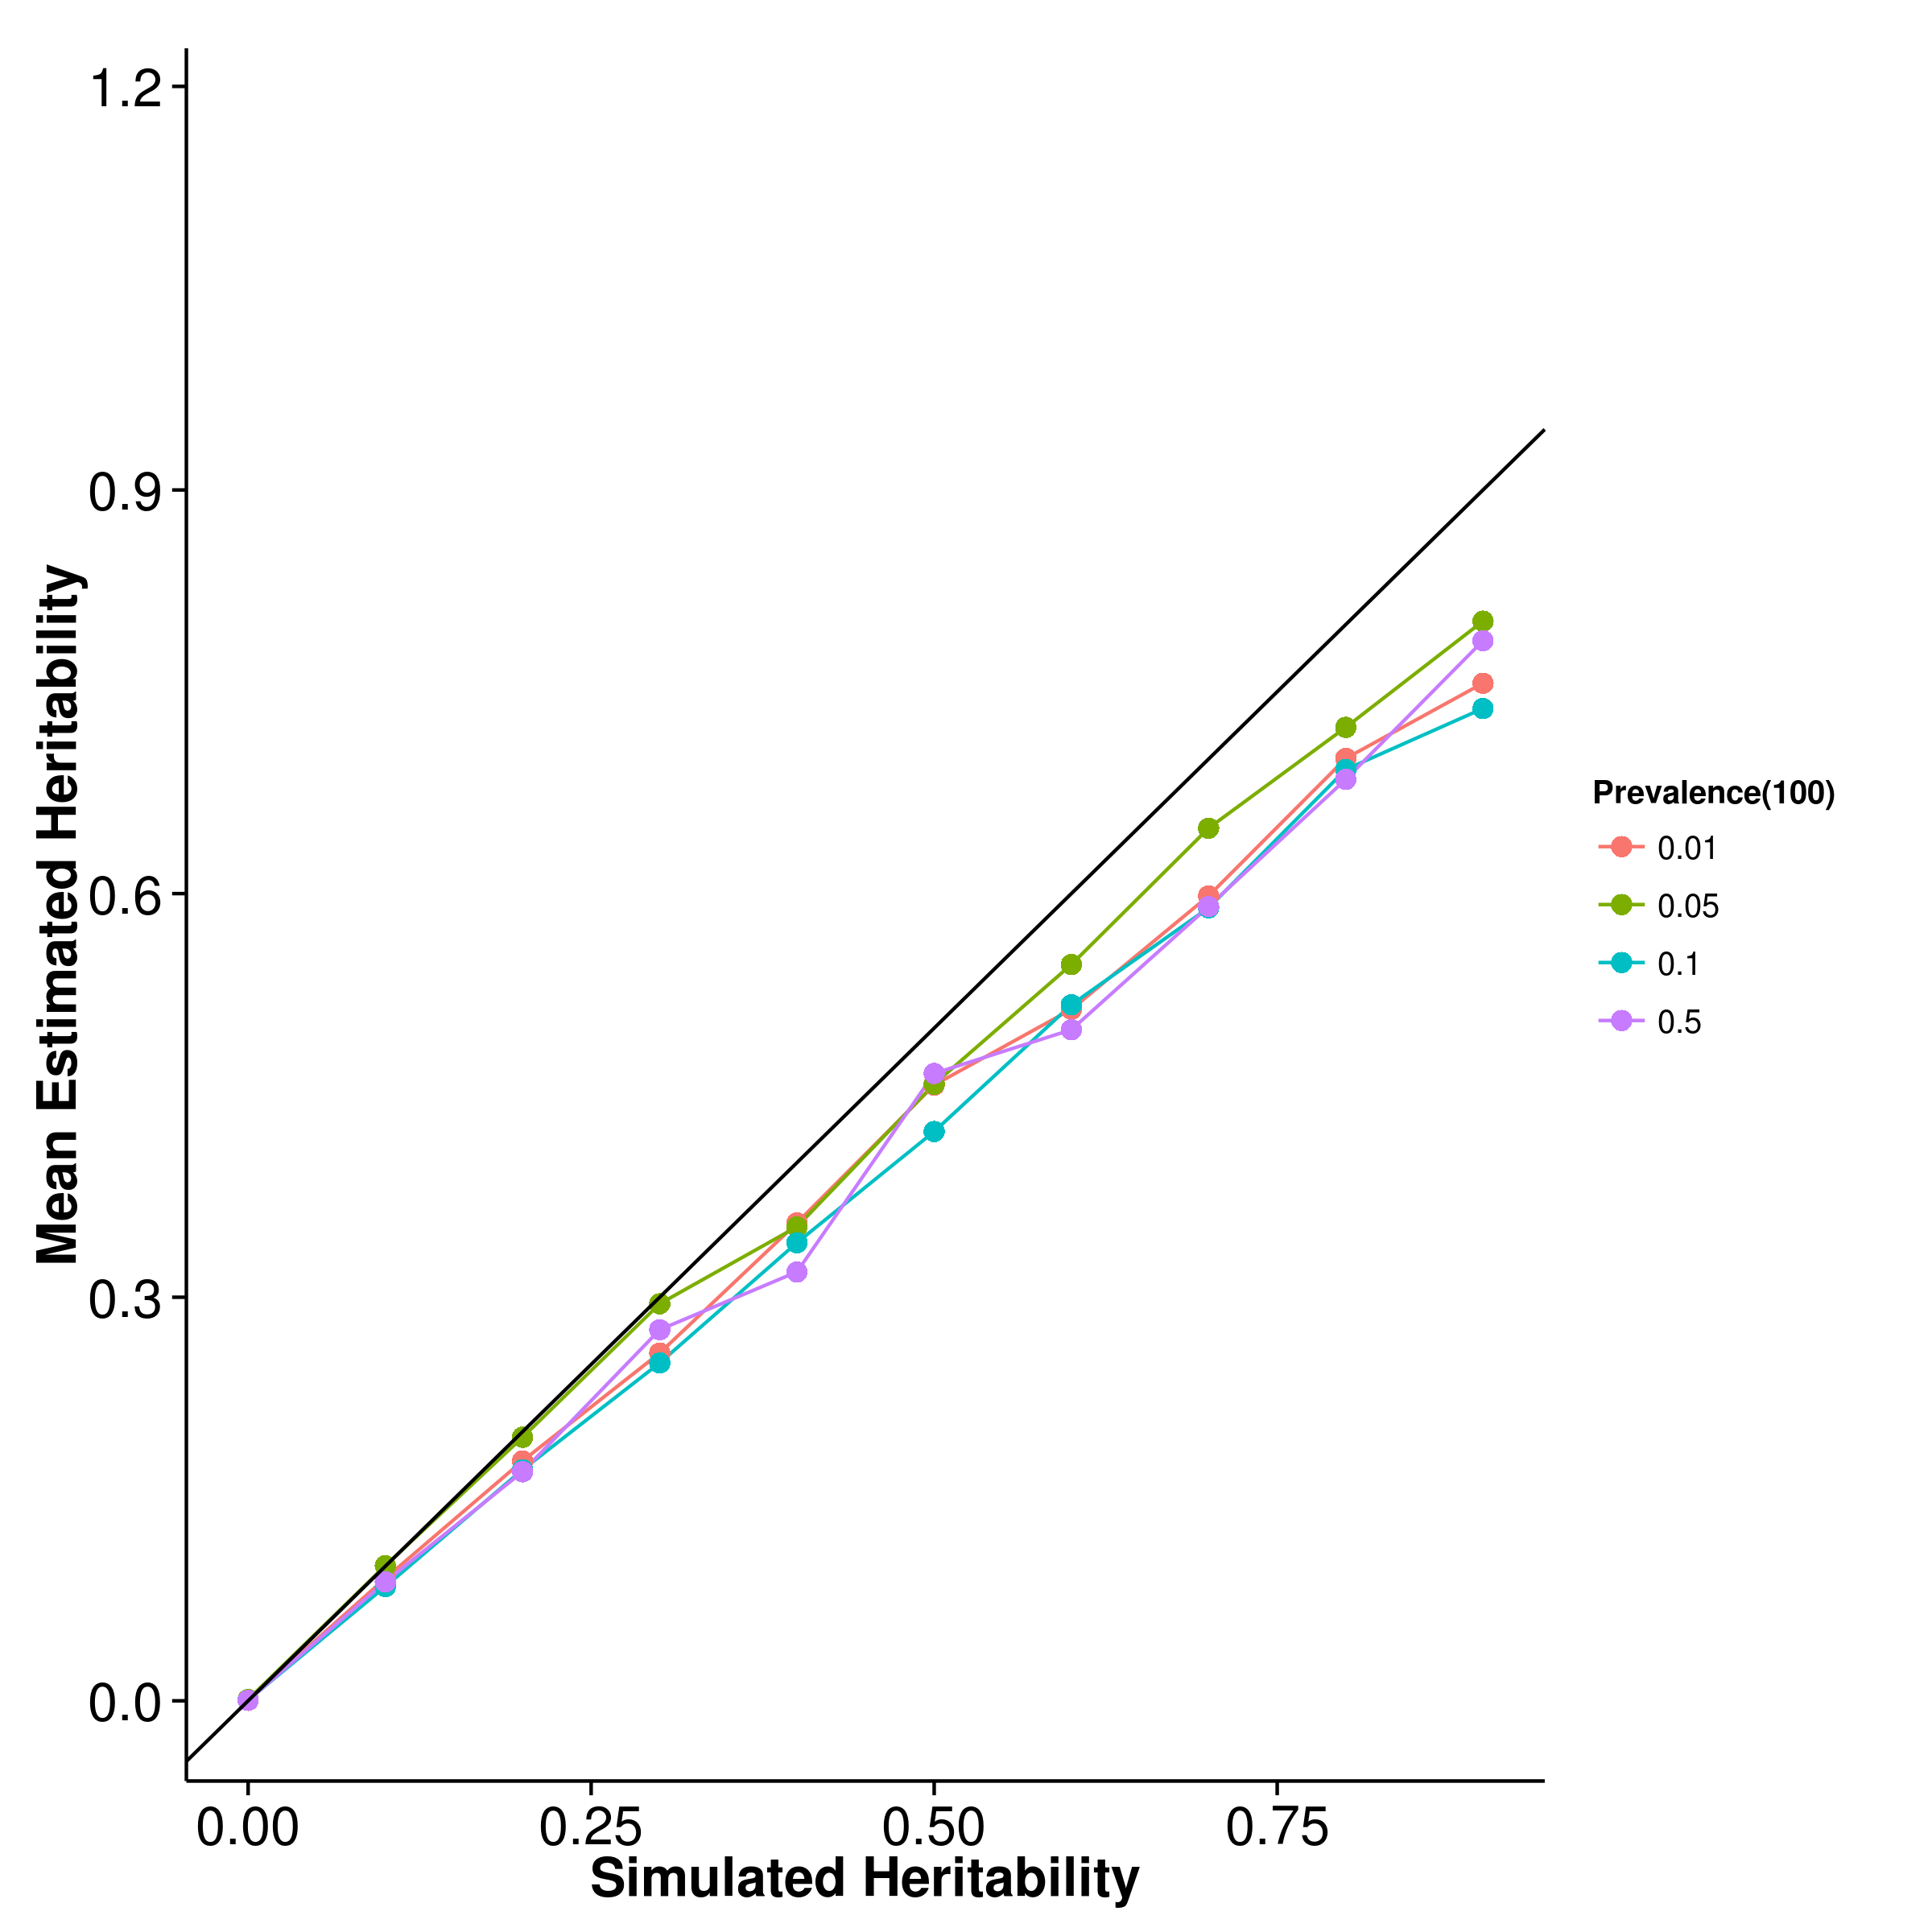
\includegraphics{figure/he_summary/cc_100c/ldscIn_CC_Rand_mean.png}}
				\label{fig:ldscInCCRandMean}
			}
			\caption[Mean of Case Control Simulation Results (100 Causal)]
			{Mean of results from case control simulation with random effect size simulation with 100 causal \glspl{SNP}.
				The bias seems to be unaffected by the number of causal \glspl{SNP} and were the same as what was observed when there were 10 or 50 causal \glspl{SNP}.
				} 
			\label{fig:CCRandMean}
		\end{figure}
		
		\begin{figure}
			\centering
			\subfloat[SHREK]{
				\scalebox{.4}{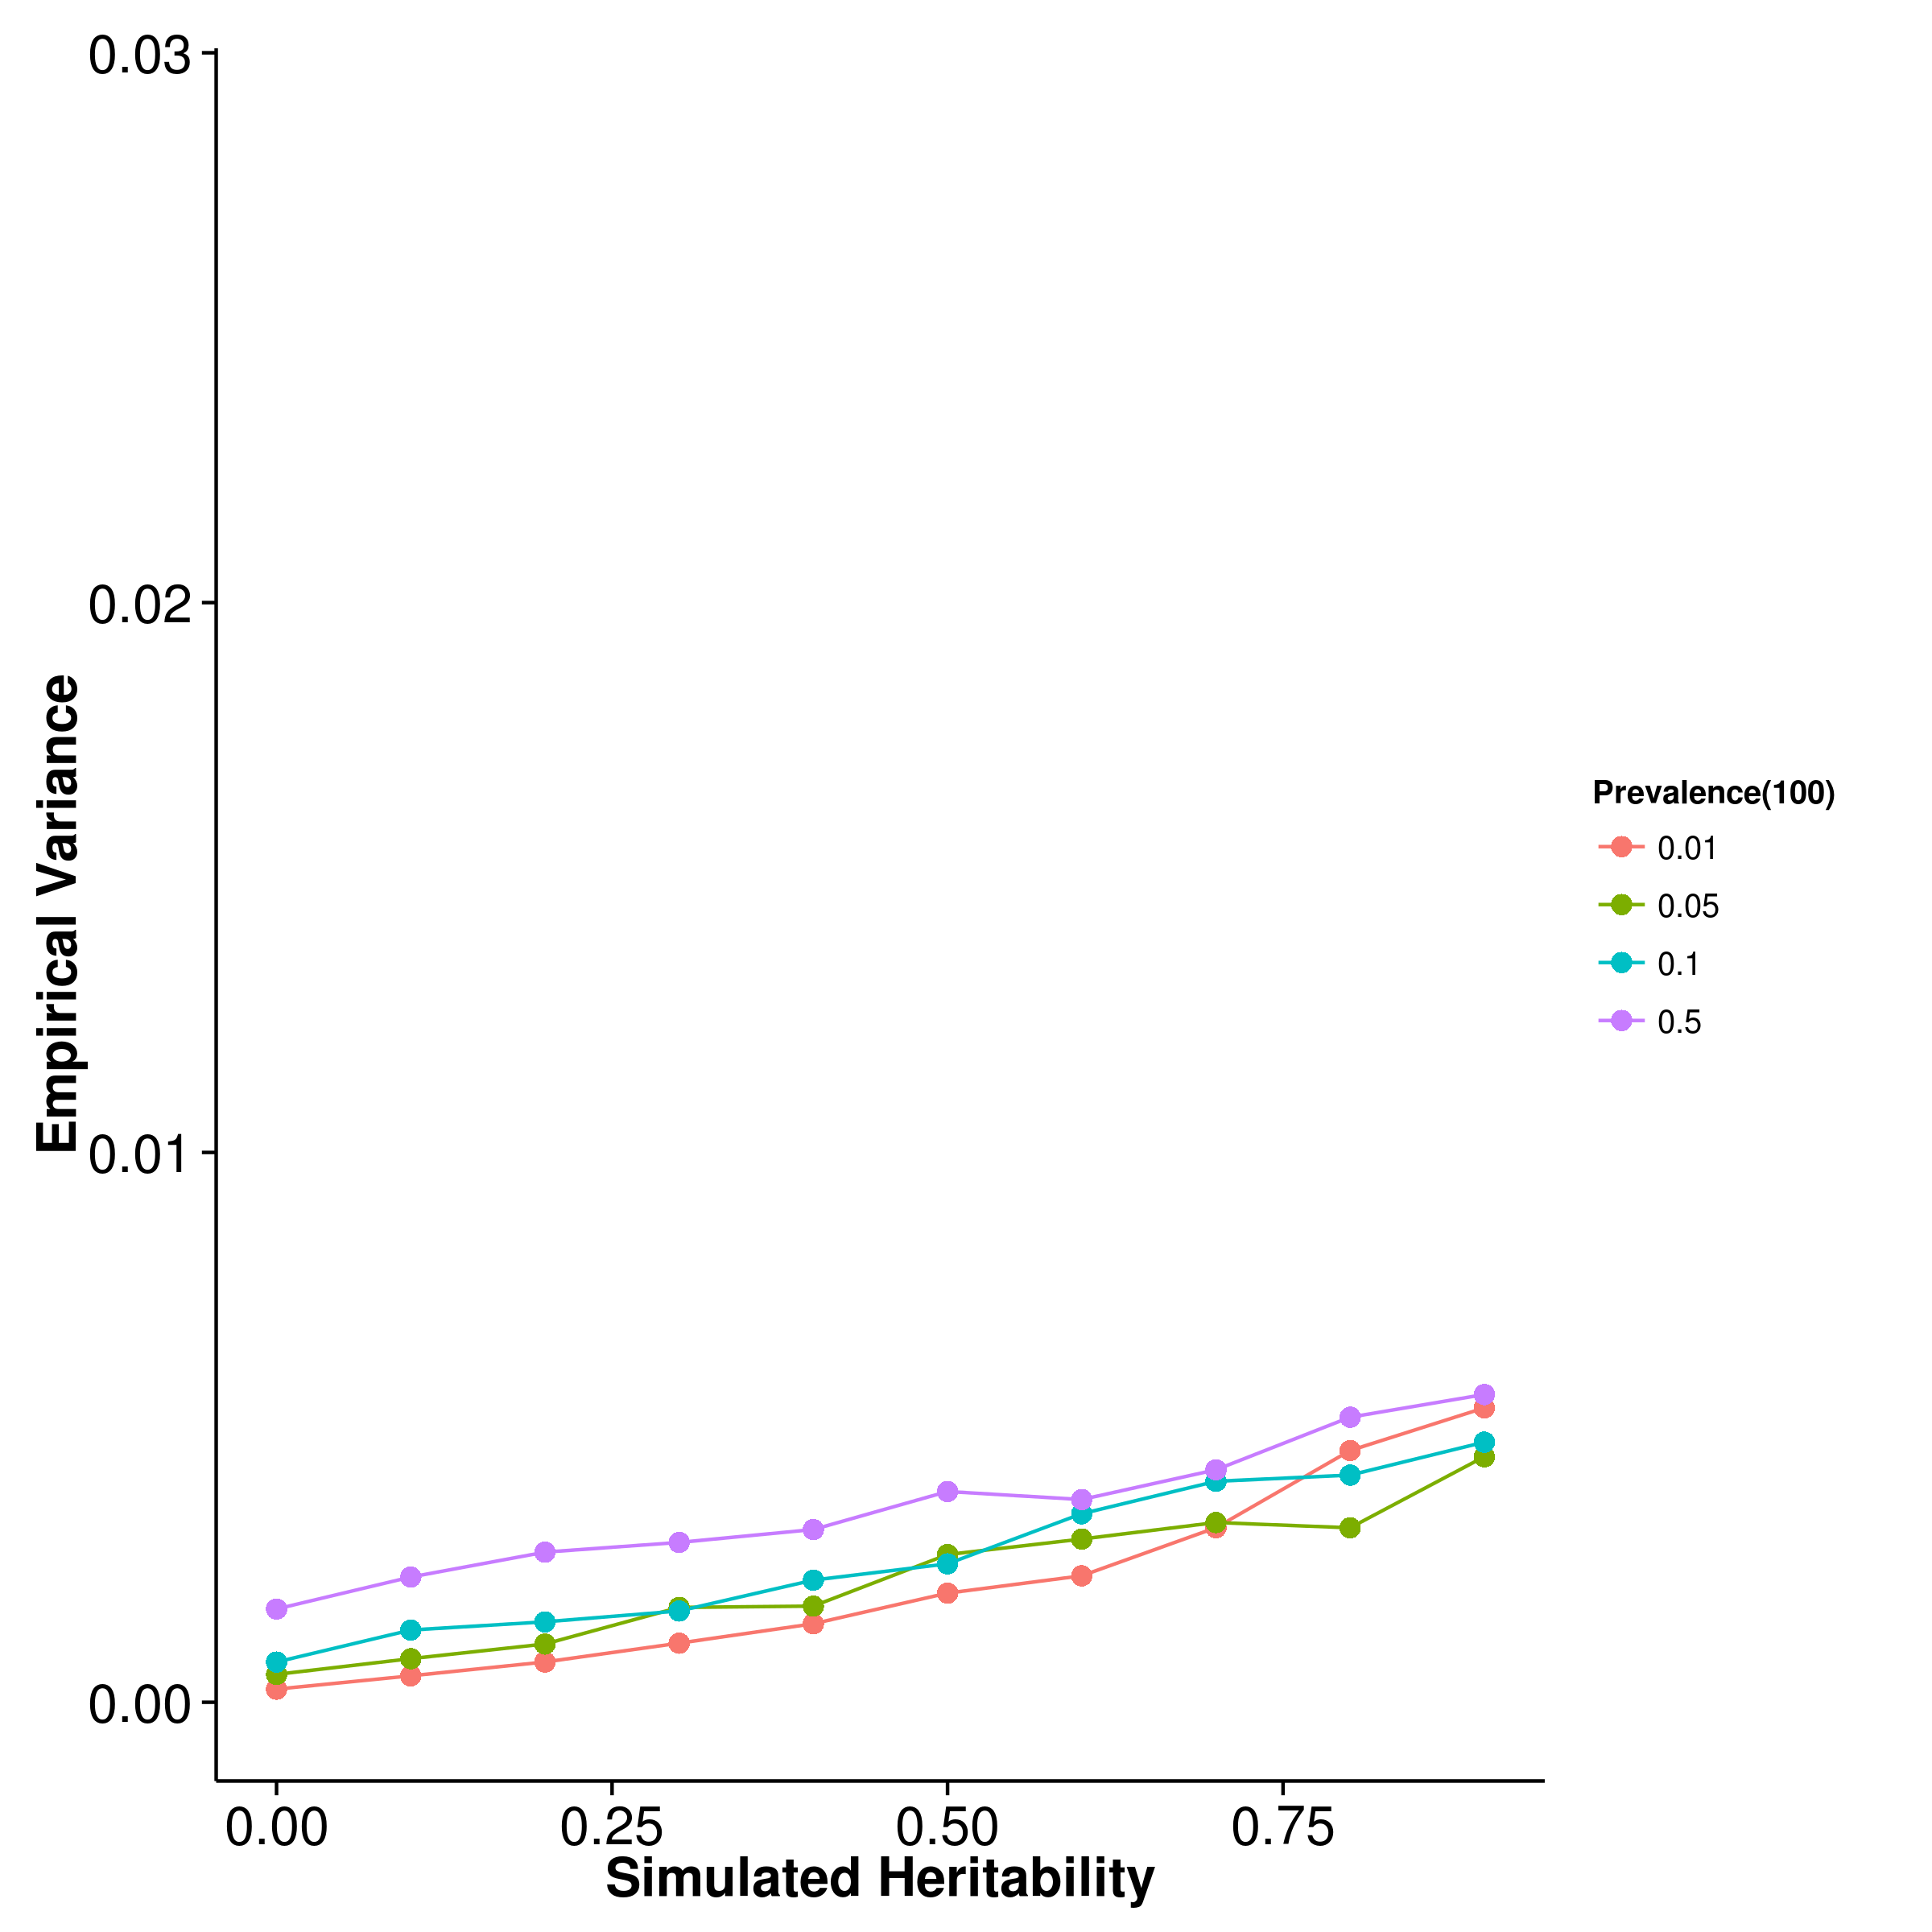
\includegraphics{figure/he_summary/cc_100c/shrek_CC_Rand_sd.png}}
				\label{fig:shrekCCRandVar}
			}
			\subfloat[GCTA]{
				\scalebox{.4}{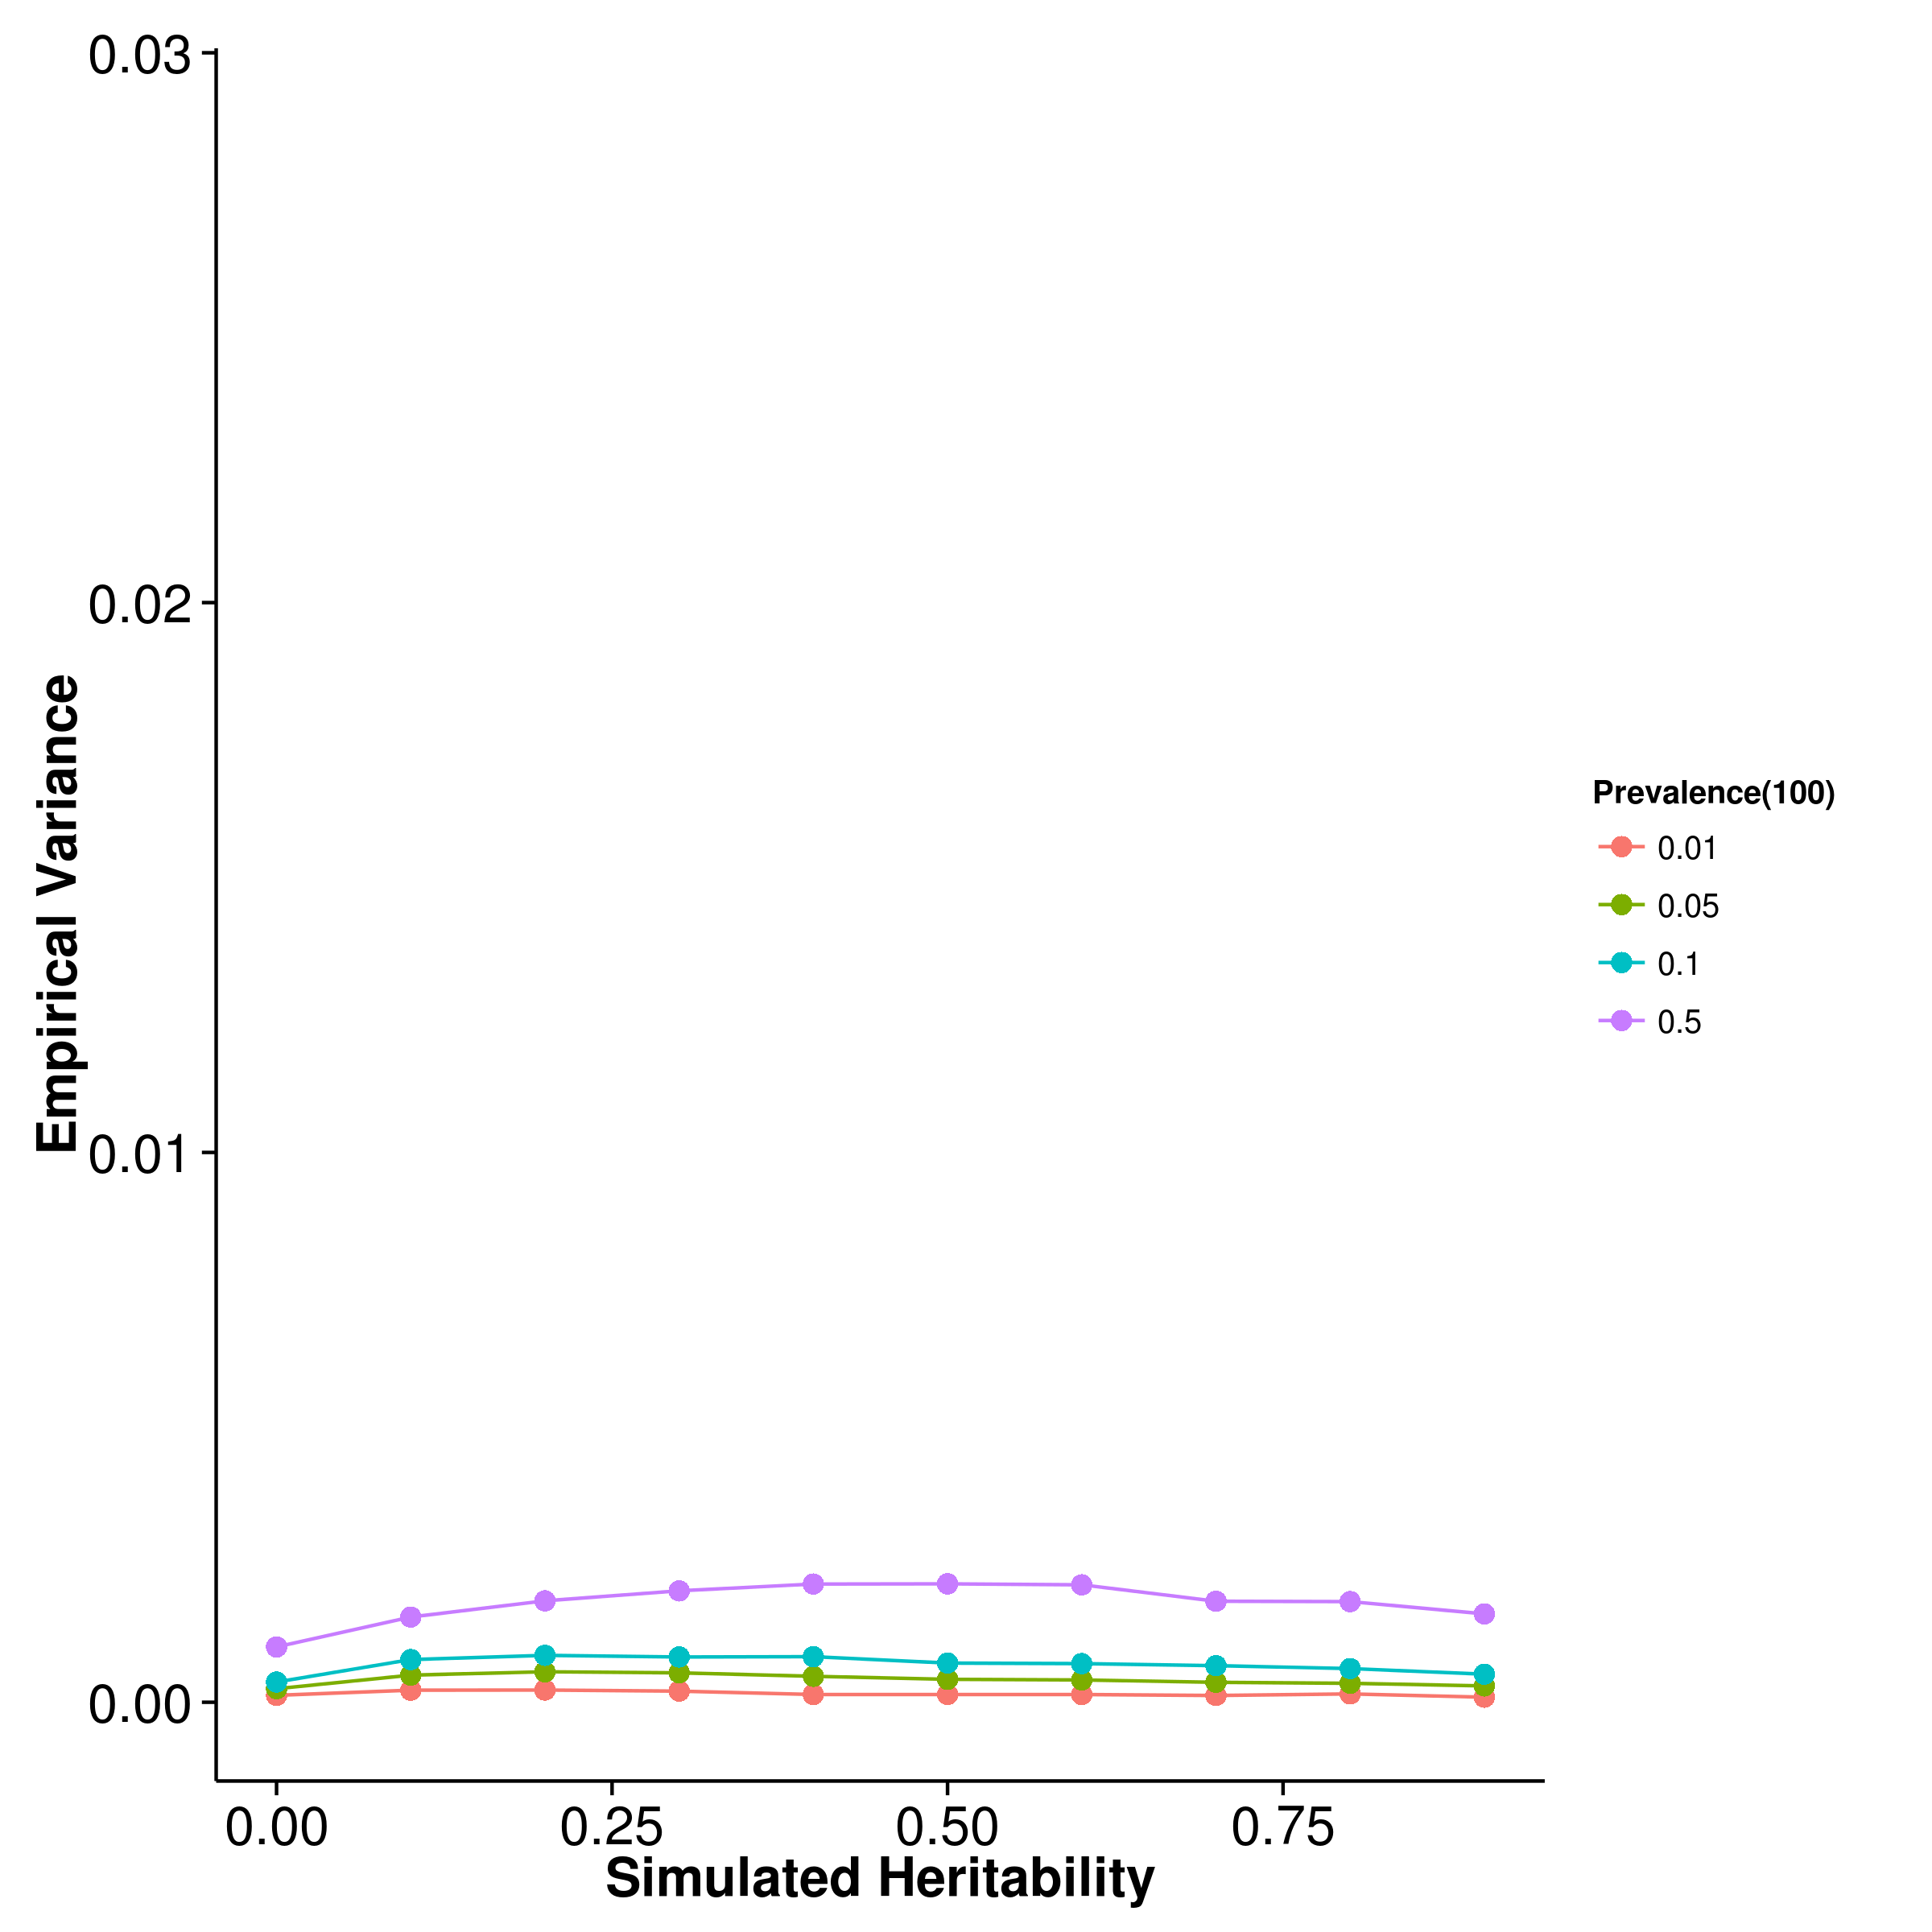
\includegraphics{figure/he_summary/cc_100c/gcta_CC_Rand_sd.png}}
				\label{fig:gctaCCRandVar}
			}\\
			\subfloat[LDSC with fix intercept]{
				\scalebox{.4}{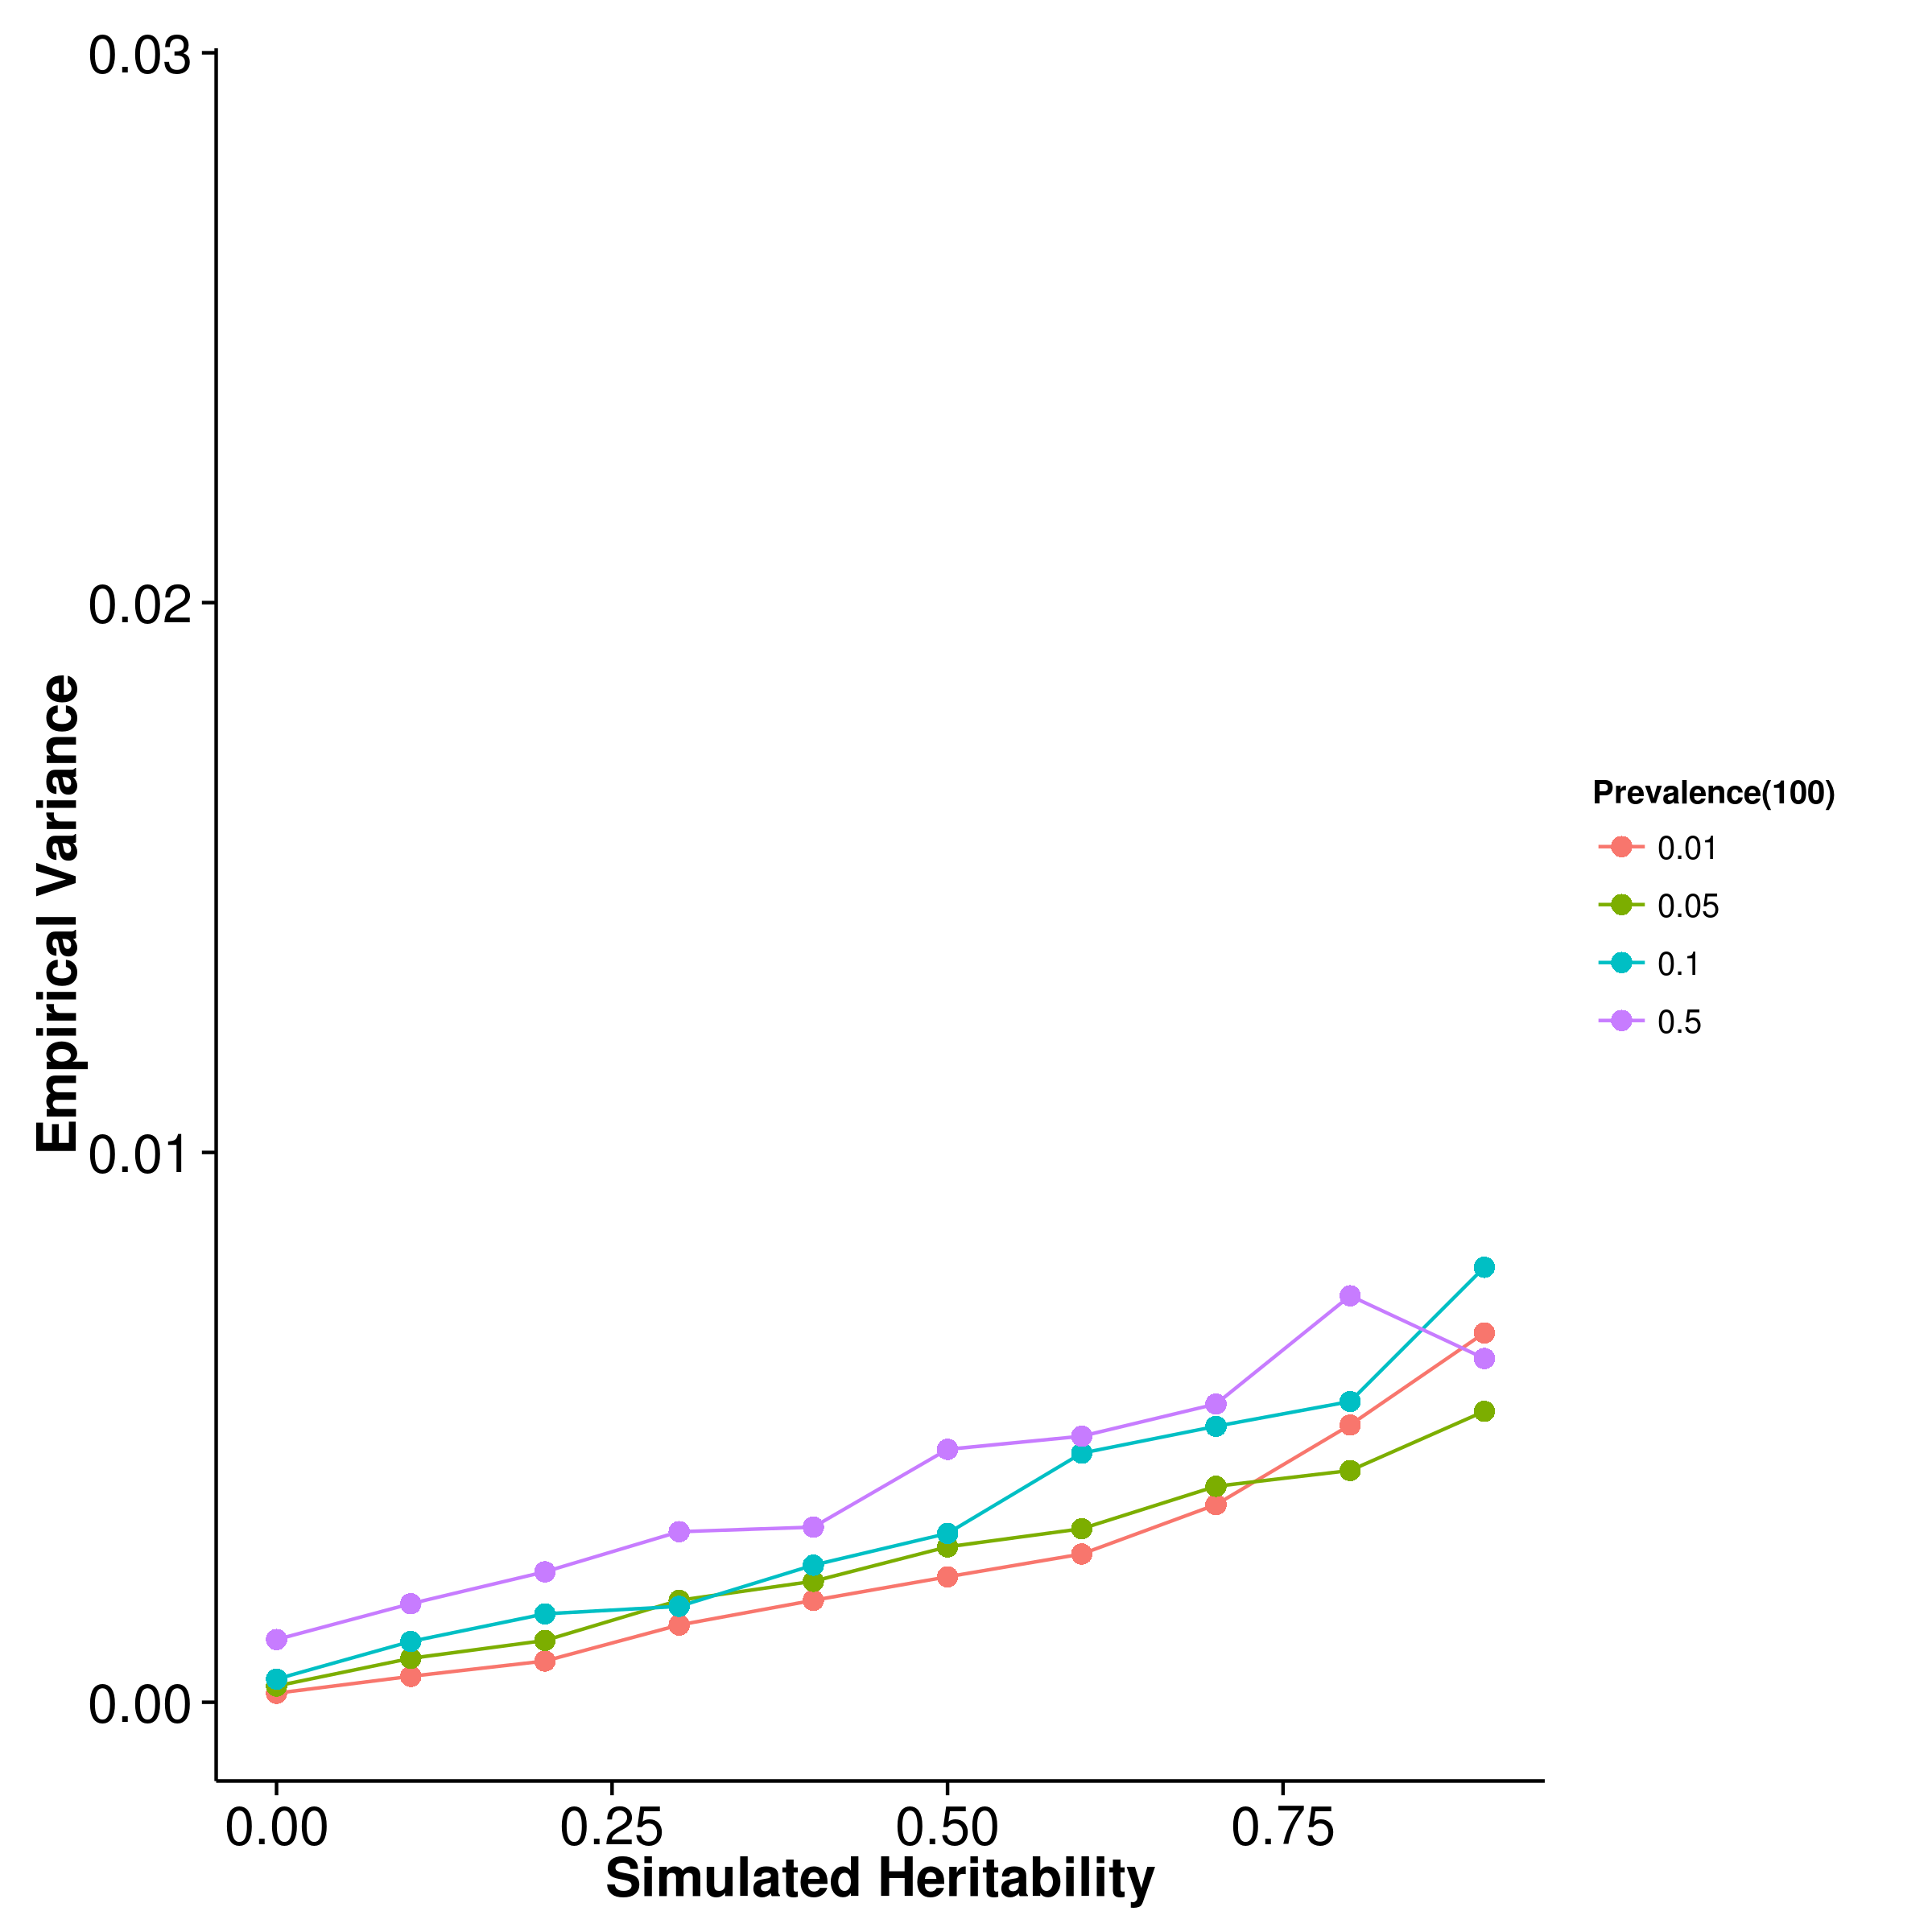
\includegraphics{figure/he_summary/cc_100c/ldsc_CC_Rand_sd.png}}
				\label{fig:ldscCCRandVar}
			}
			\subfloat[LDSC with intercept estimation]{
				
				\scalebox{.4}{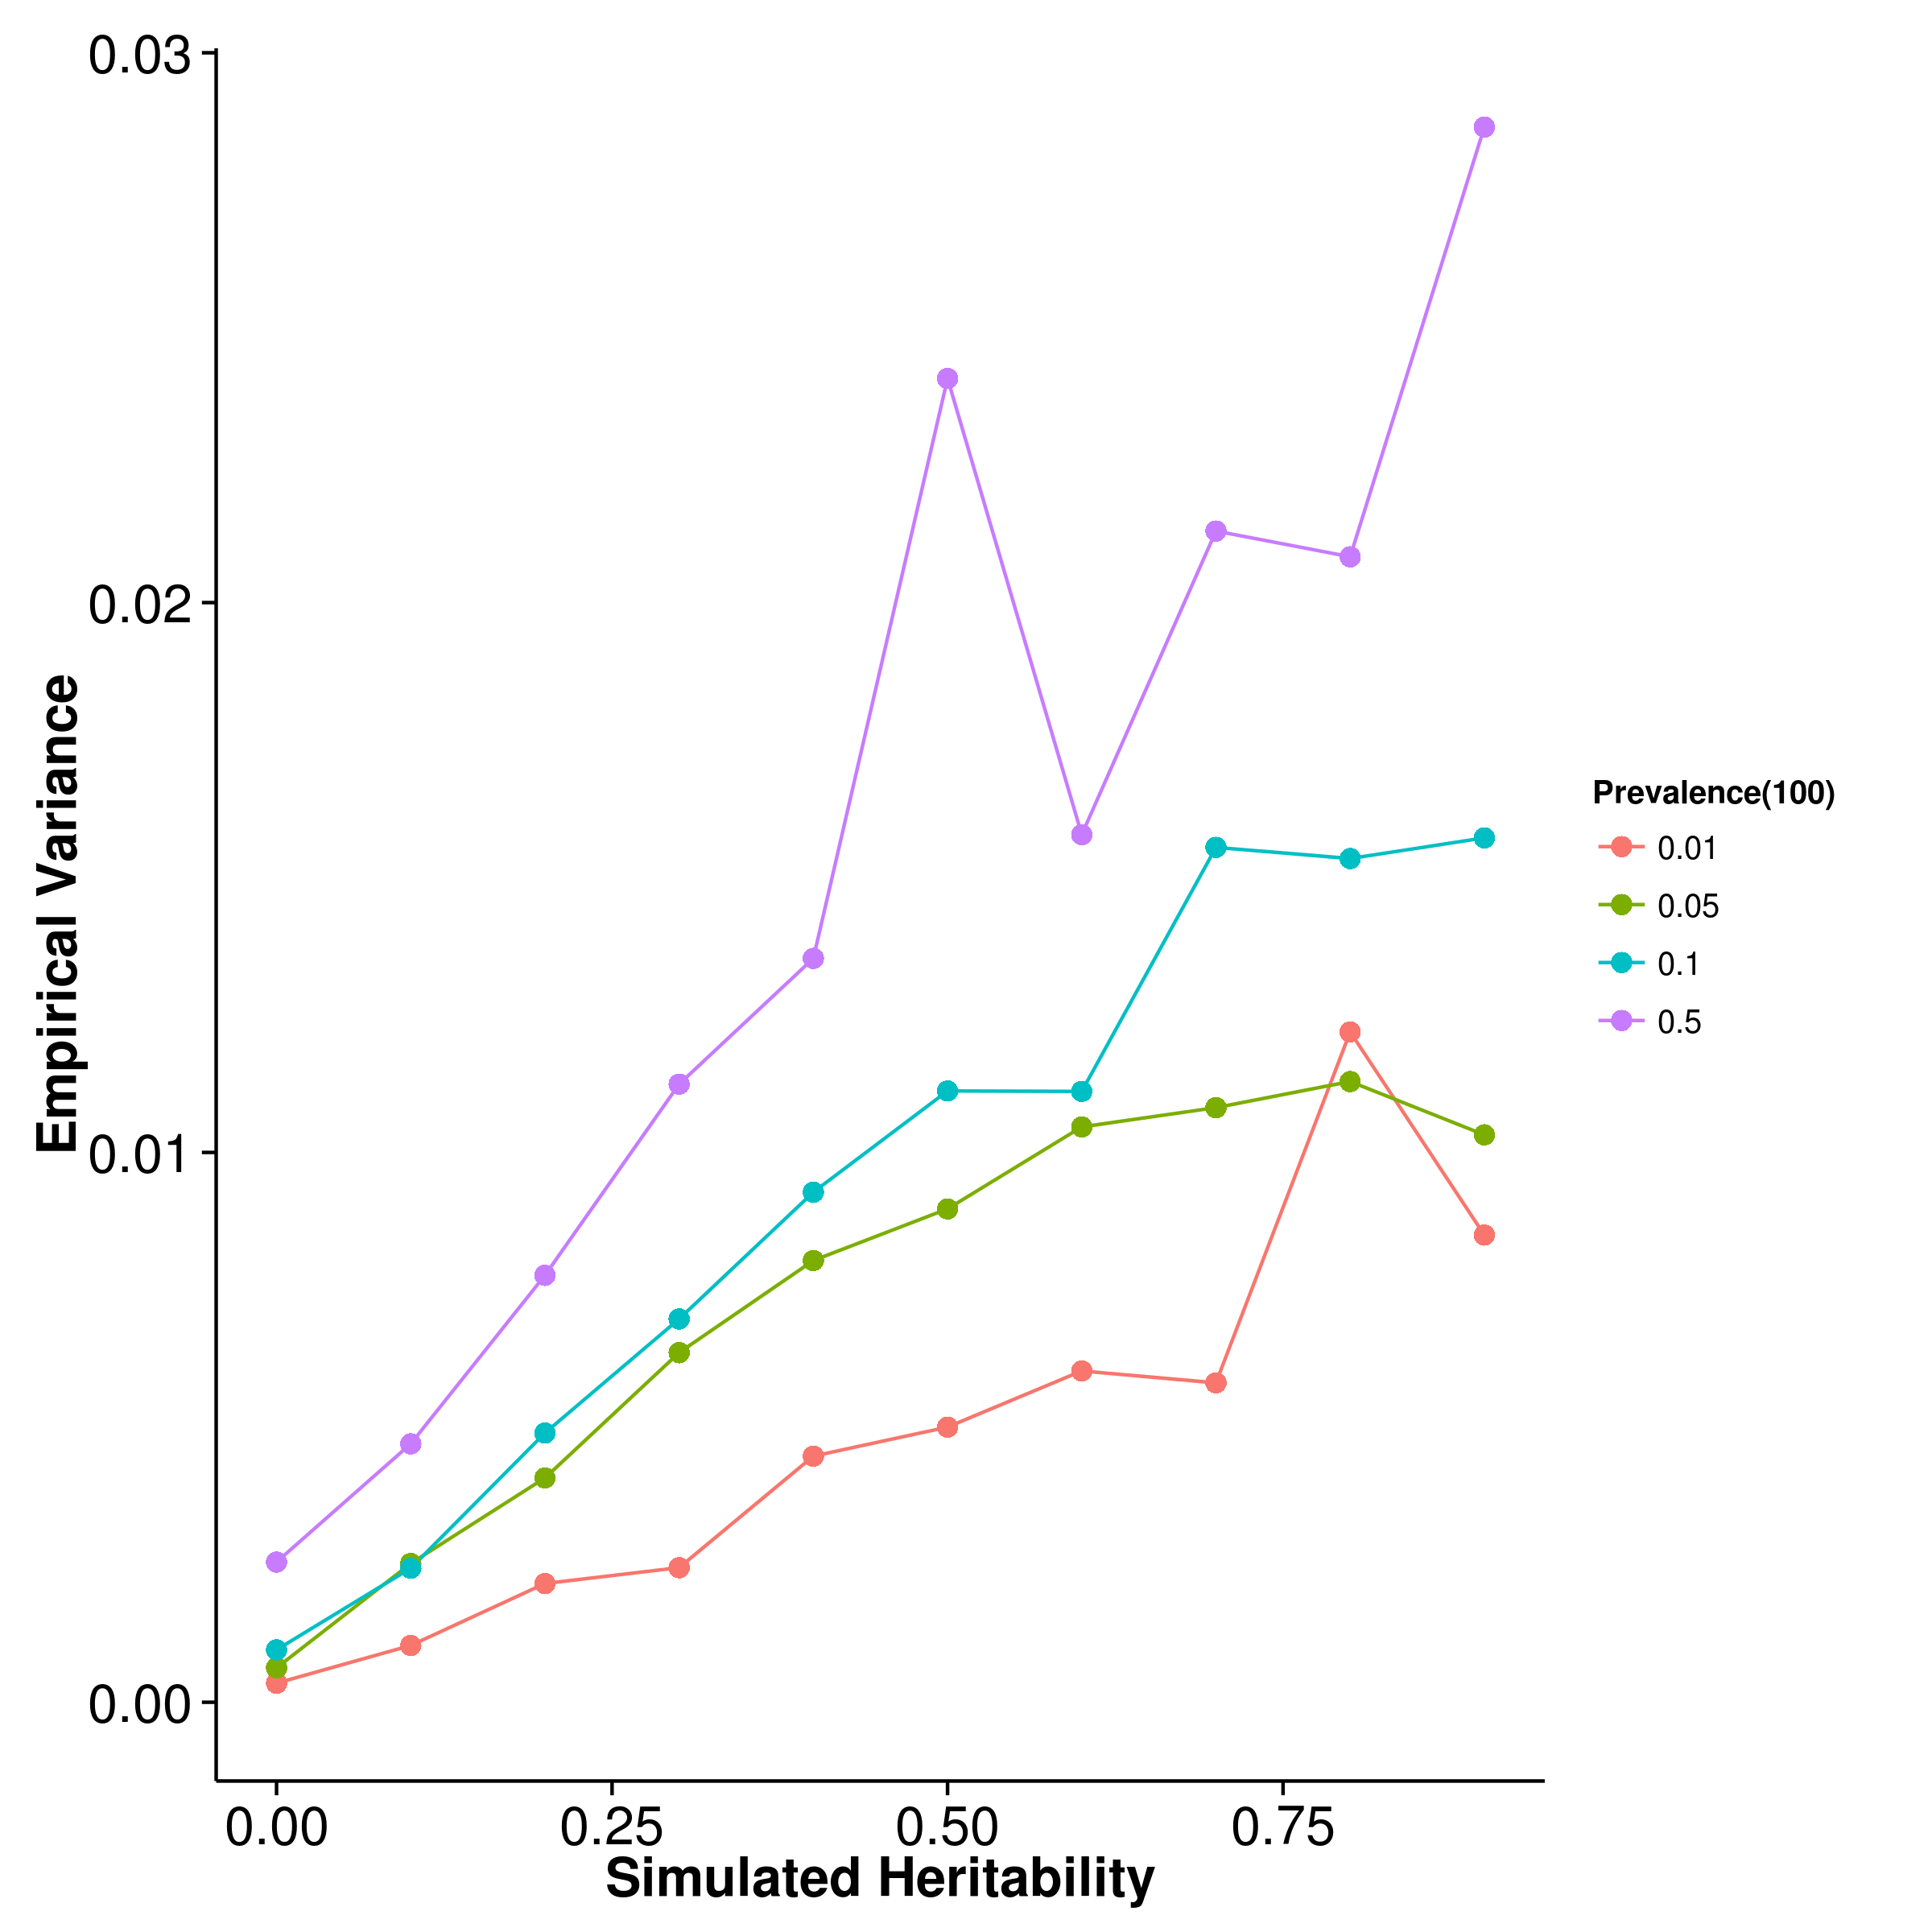
\includegraphics{figure/he_summary/cc_100c/ldscIn_CC_Rand_sd.png}}
				\label{fig:ldscInCCRandVar}
			}
			\caption[Variance of Case Control Simulation Results (100 Causal)]
			{Variance of results from case control simulation with random effect size simulation with 100 causal \glspl{SNP}.
				As the number of causal \glspl{SNP} increased to 100, the relationship between the population prevalence and the empirical variance of the algorithms become clear where as the population prevalence increases, the empirical variance of all algorithm increases.
				Again, \gls{ldsc} with intercept estimation has the largest variation of all the algorithms and the empirical variance of \gls{ldsc} with fix intercept is only slightly higher than that of \gls{shrek}.
			} 
			\label{fig:CCRandVar}
		\end{figure}
		
		
		\begin{figure}
			\centering
			\subfloat[SHREK]{
				\scalebox{.4}{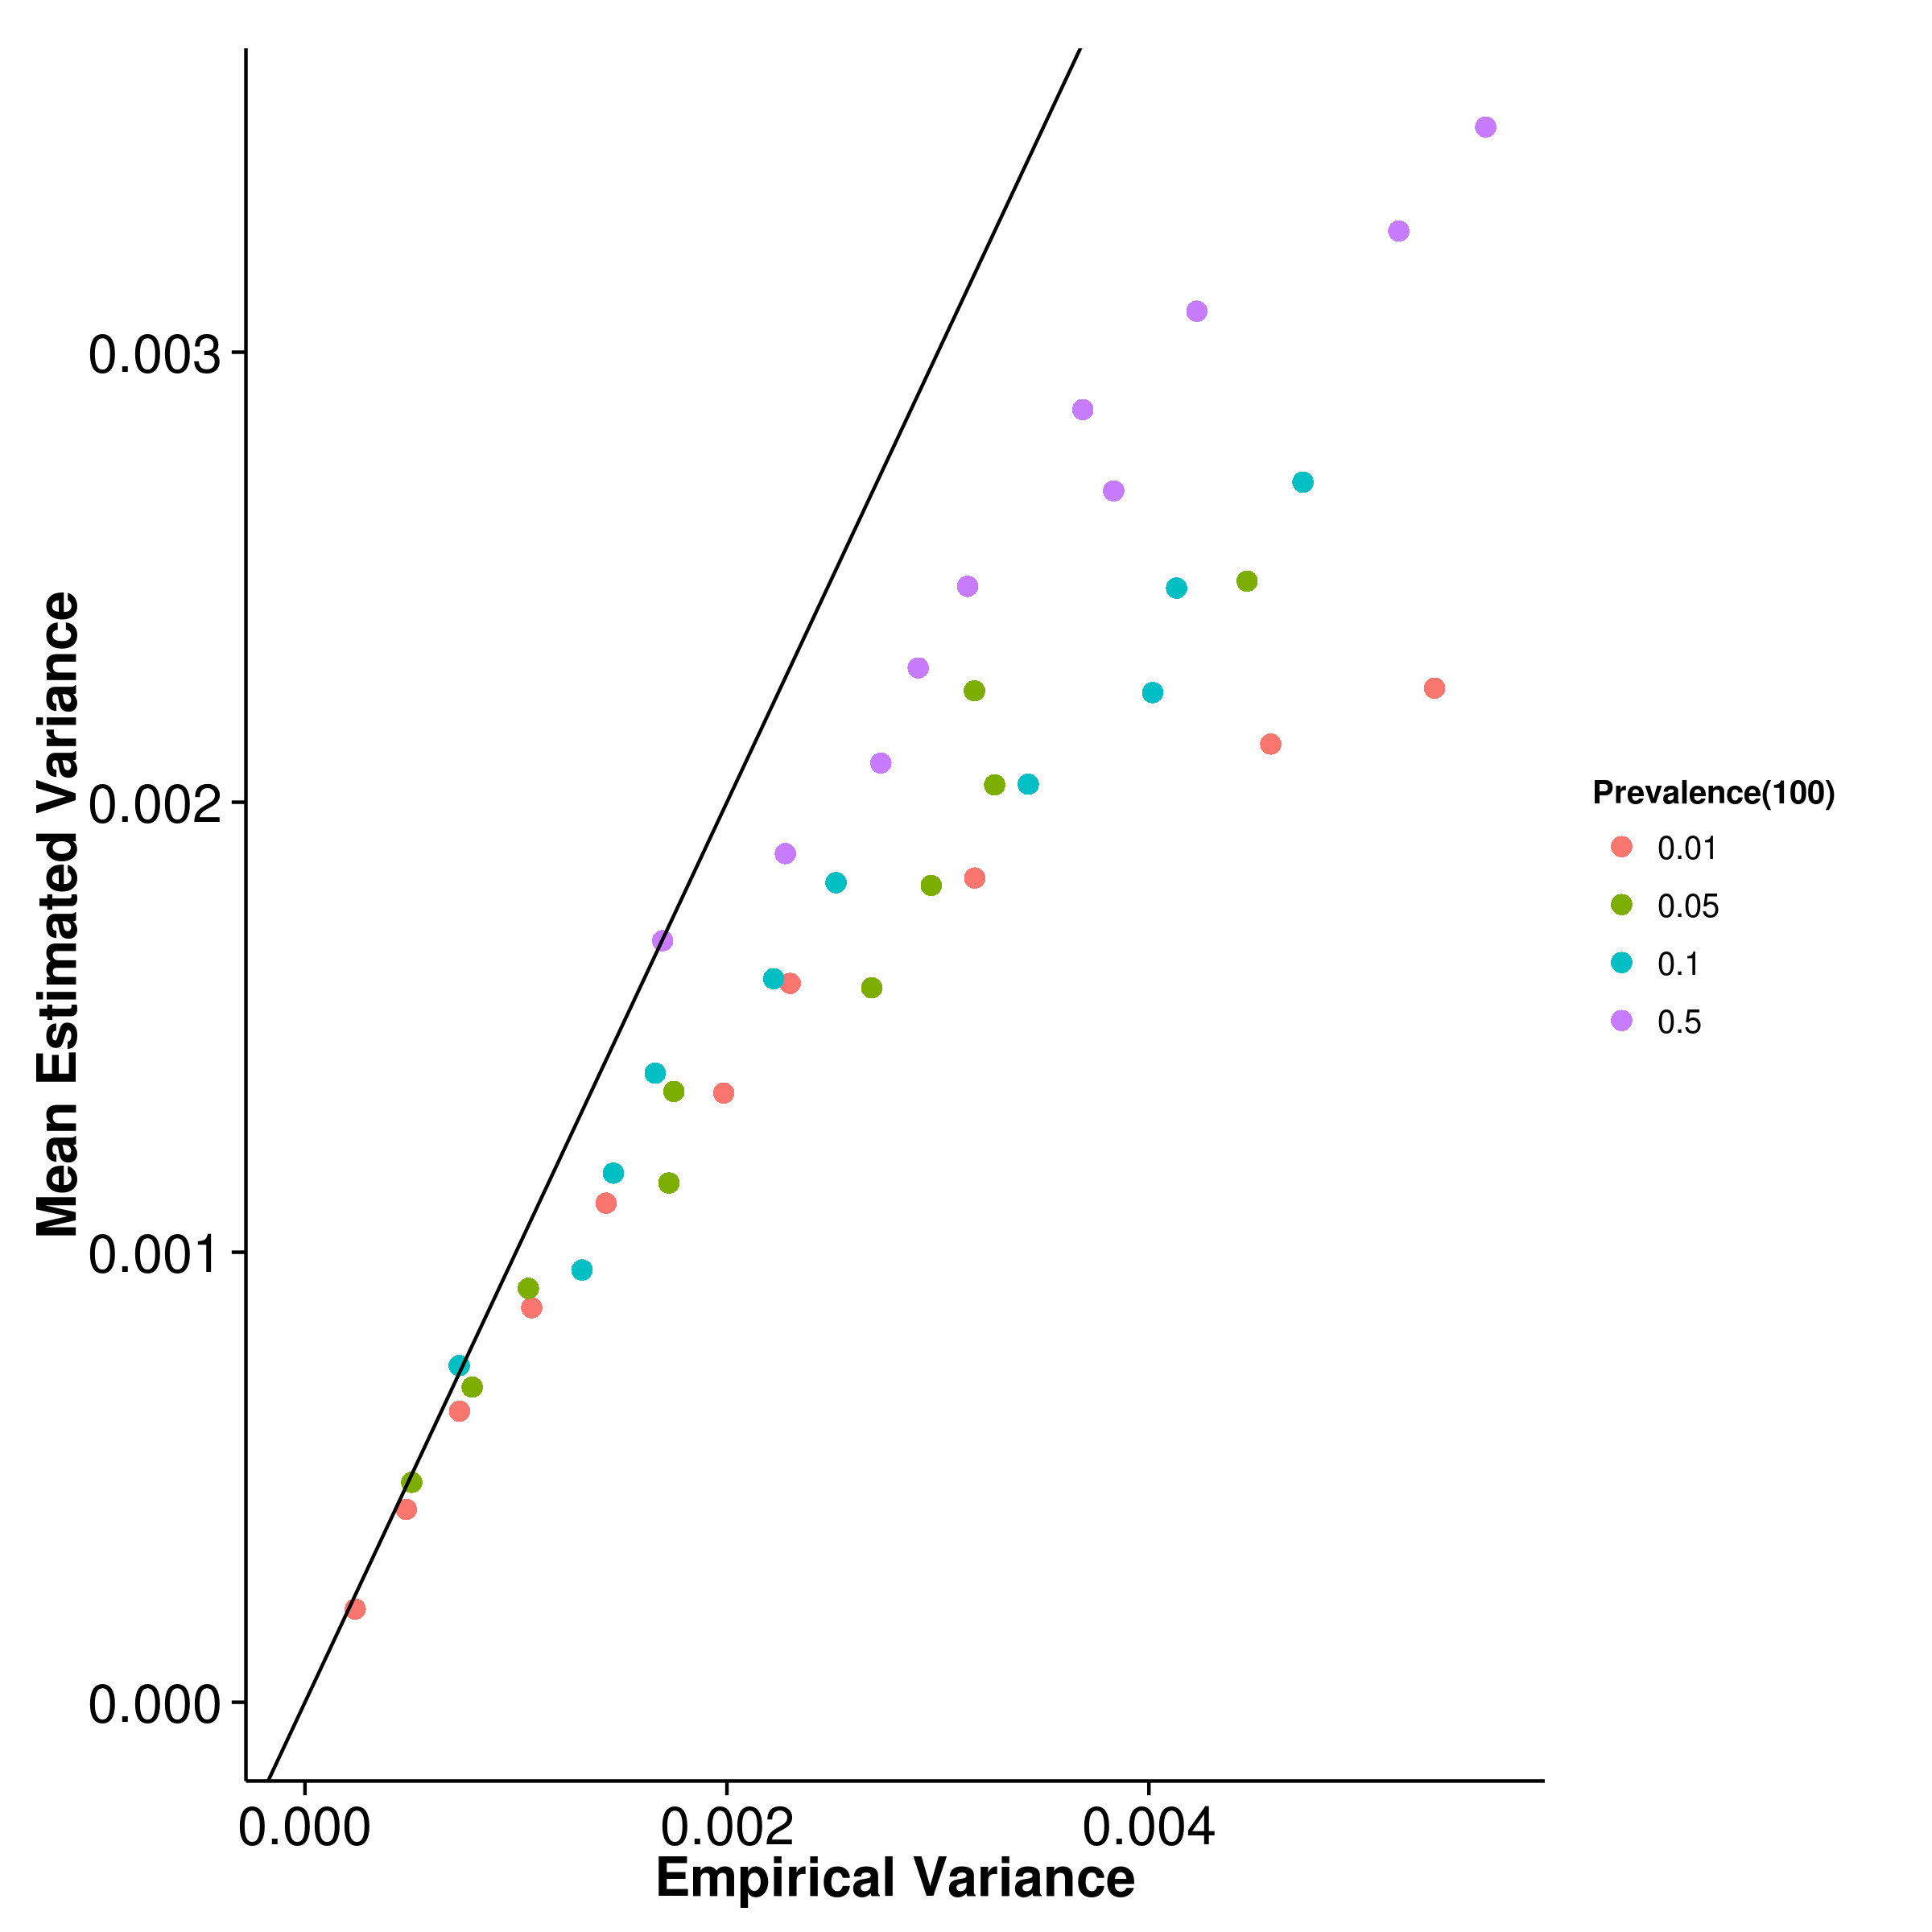
\includegraphics{figure/he_summary/cc_100c/shrek_CC_Rand_sdCom.png}}
				\label{fig:shrekCCRandVarCom}
			}
			\subfloat[GCTA]{
				\scalebox{.4}{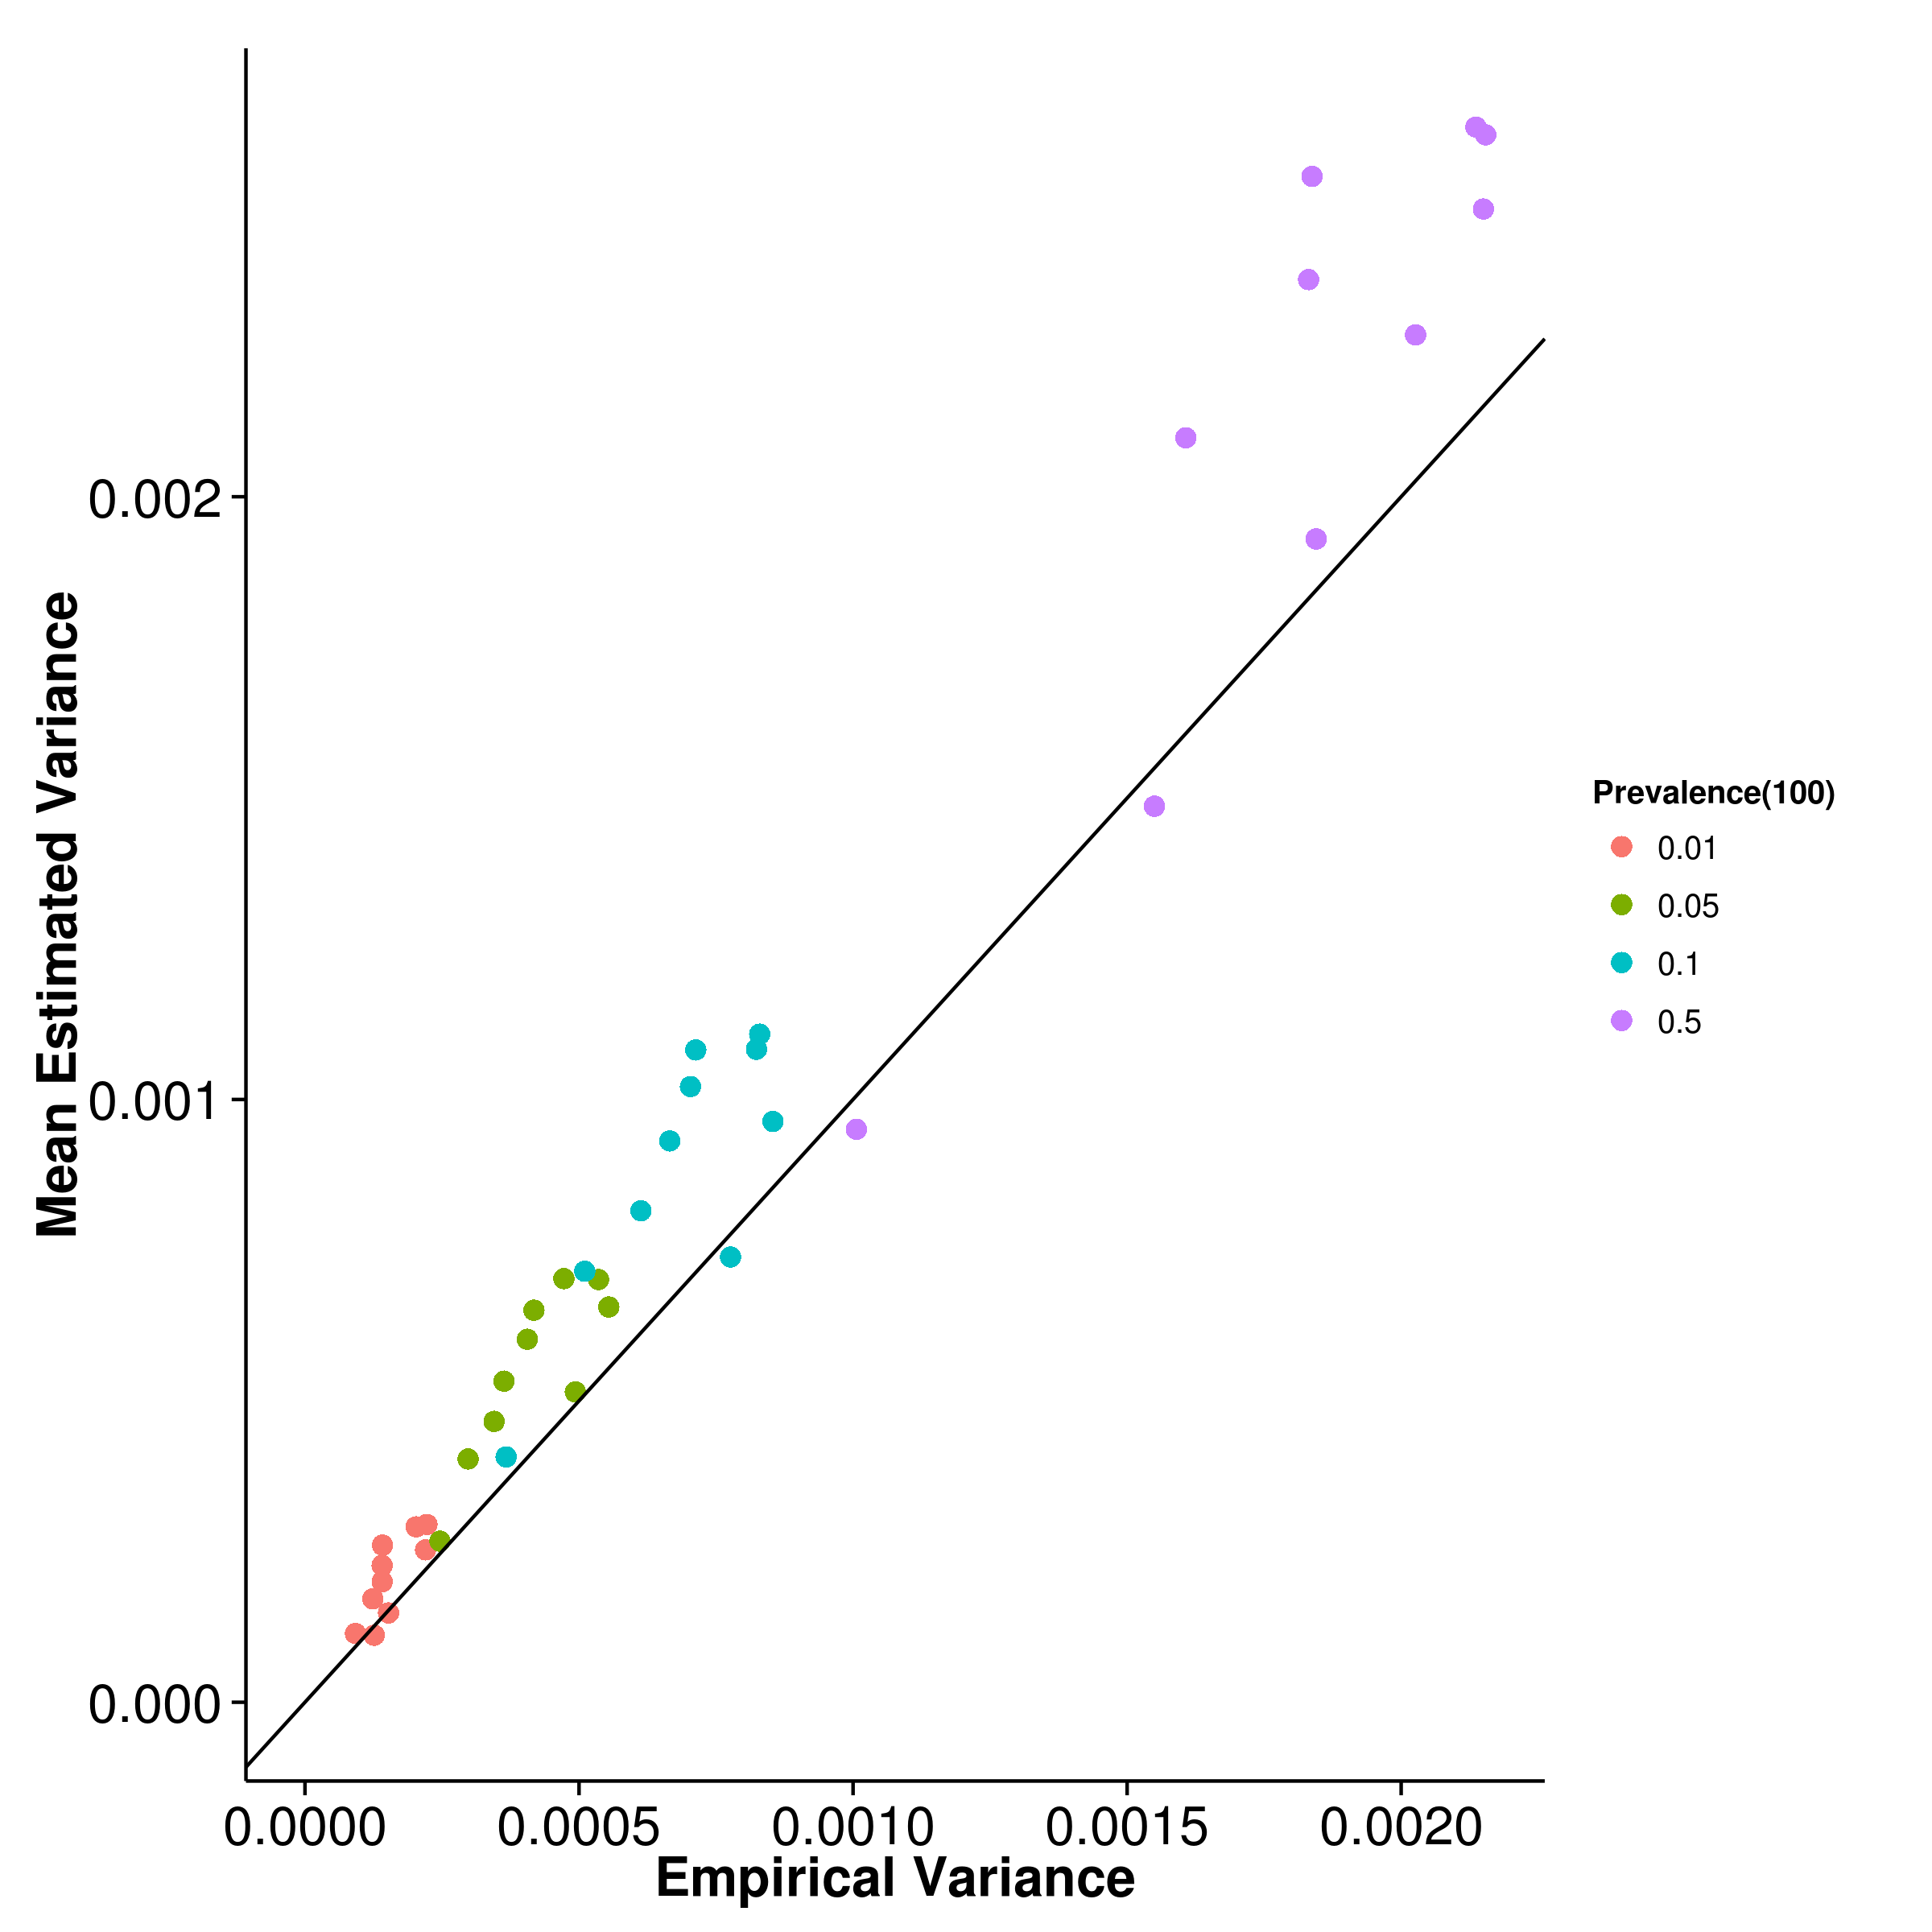
\includegraphics{figure/he_summary/cc_100c/gcta_CC_Rand_sdCom.png}}
				\label{fig:gctaCCRandVarCom}
			}\\
			\subfloat[LDSC with fix intercept]{
				\scalebox{.4}{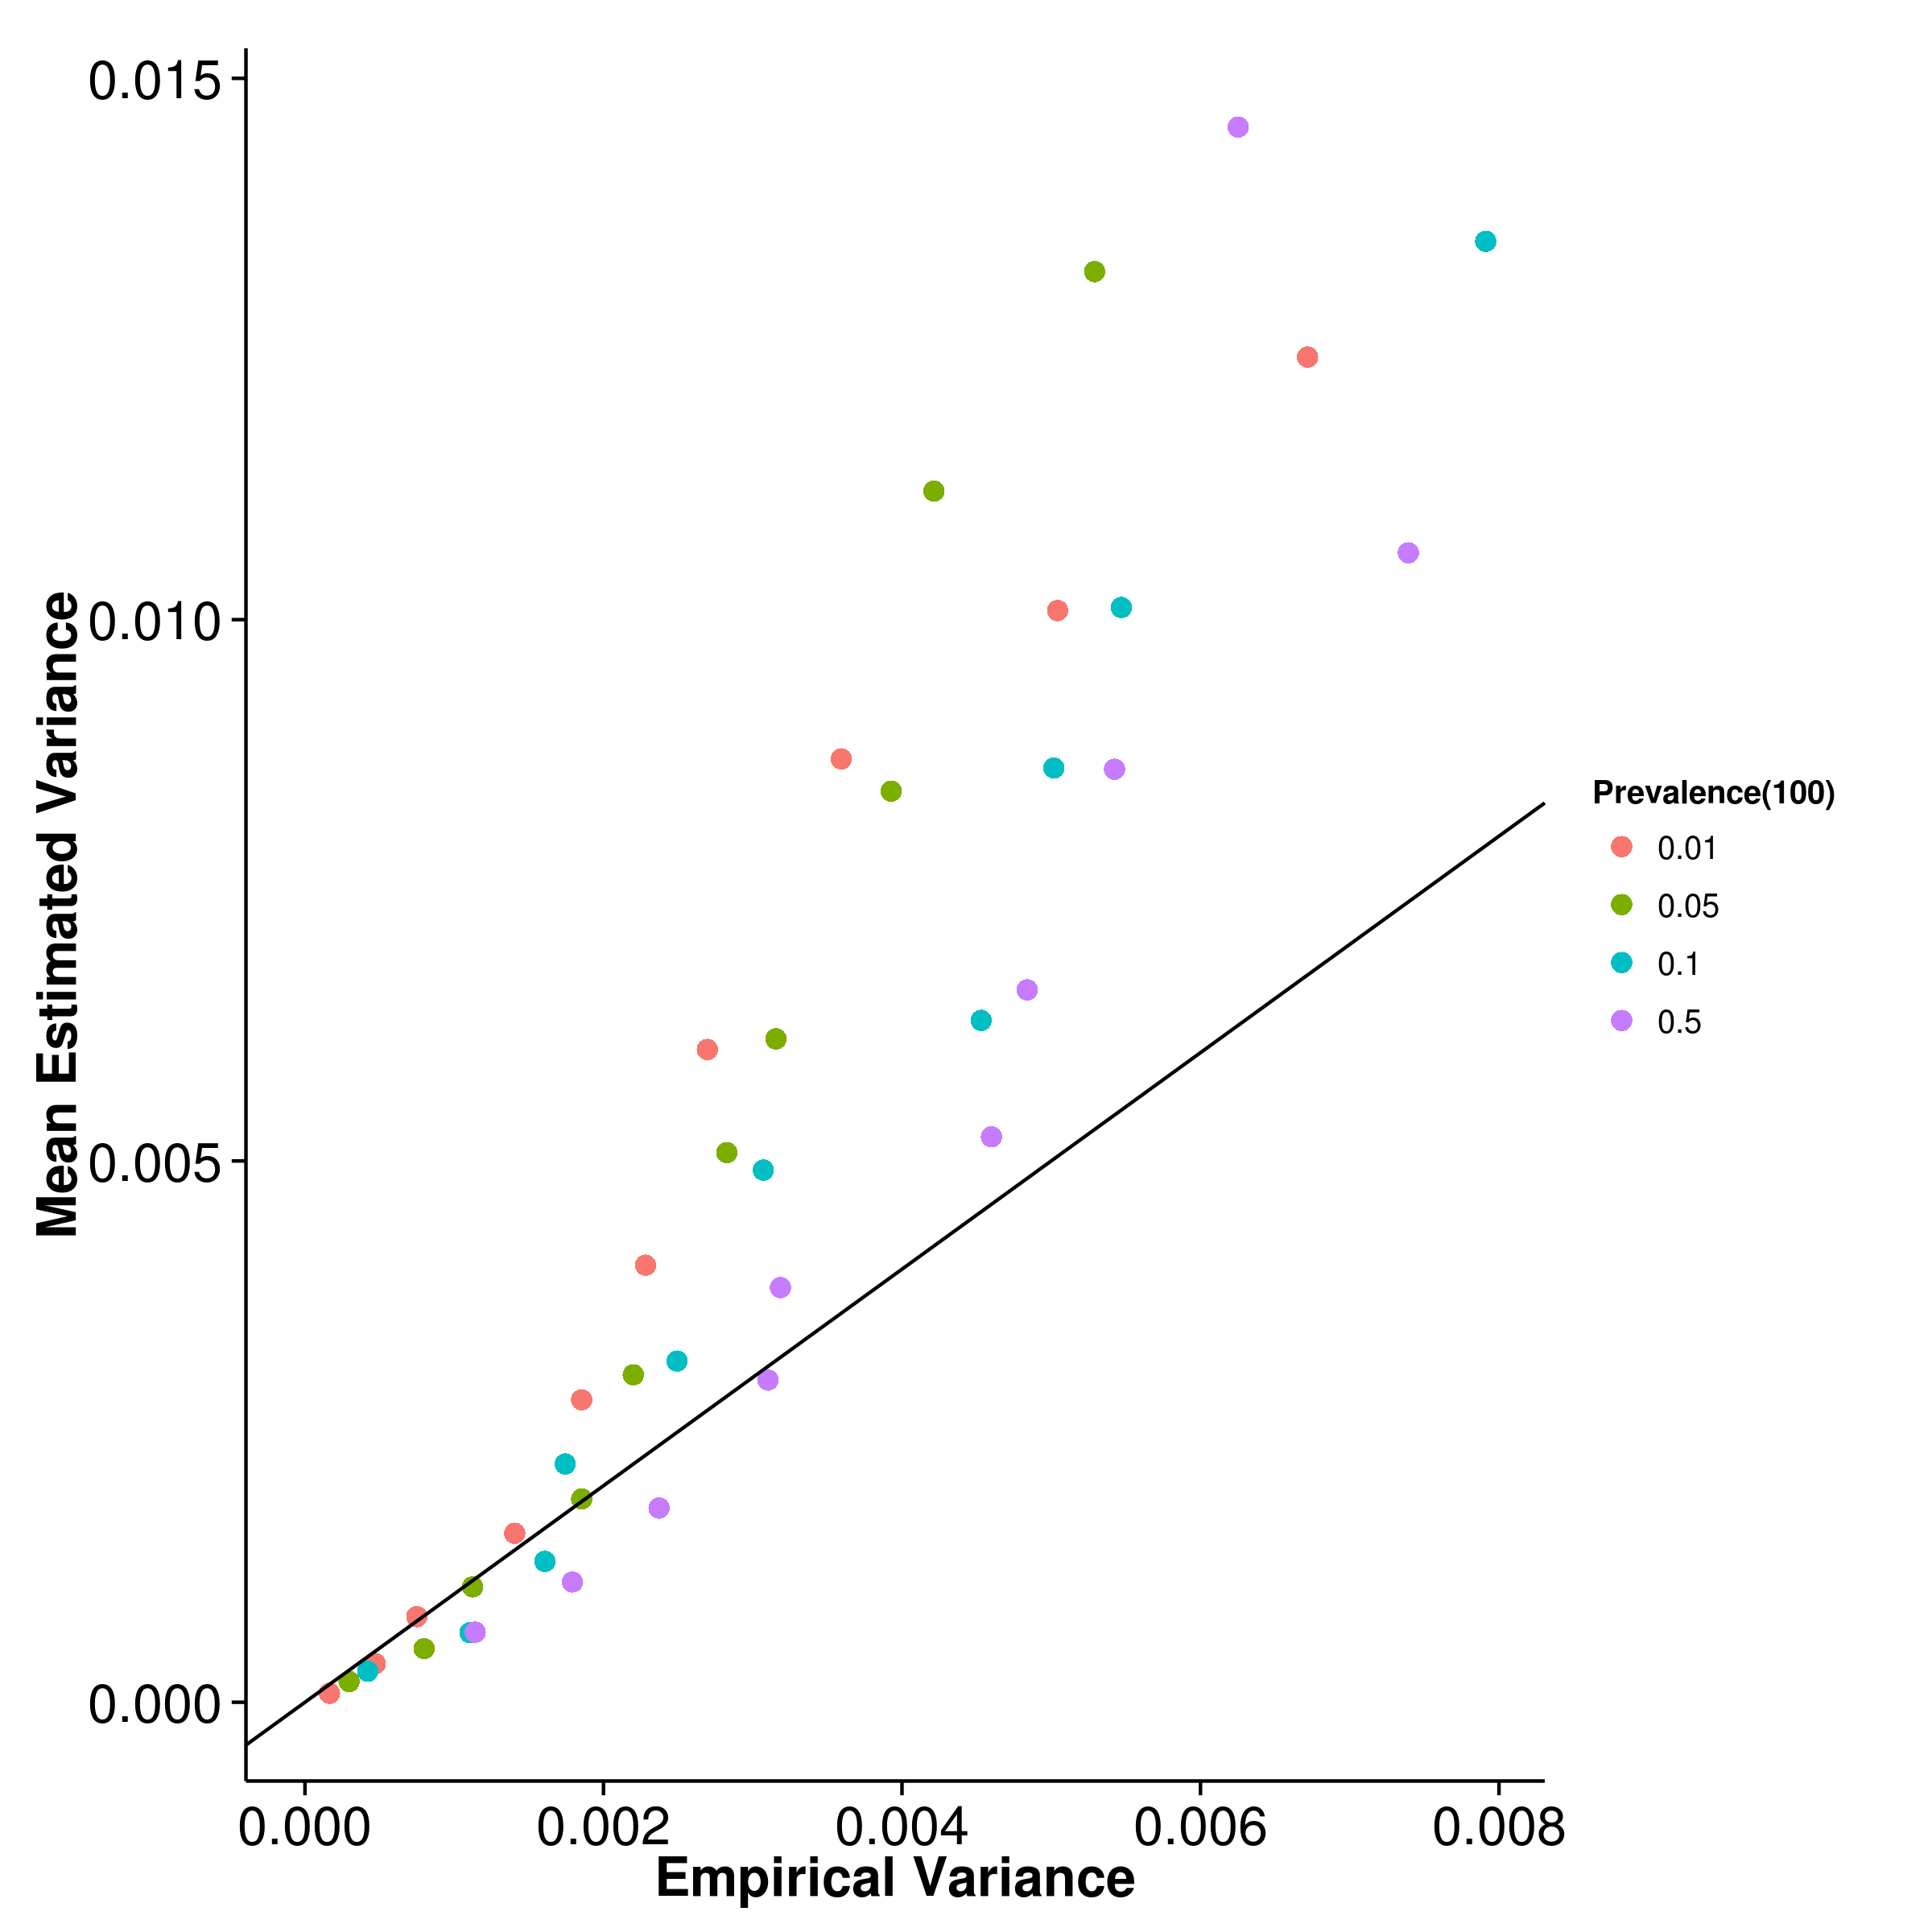
\includegraphics{figure/he_summary/cc_100c/ldsc_CC_Rand_sdCom.png}}
				\label{fig:ldscCCRandVarCom}
			}
			\subfloat[LDSC with intercept estimation]{
				
				\scalebox{.4}{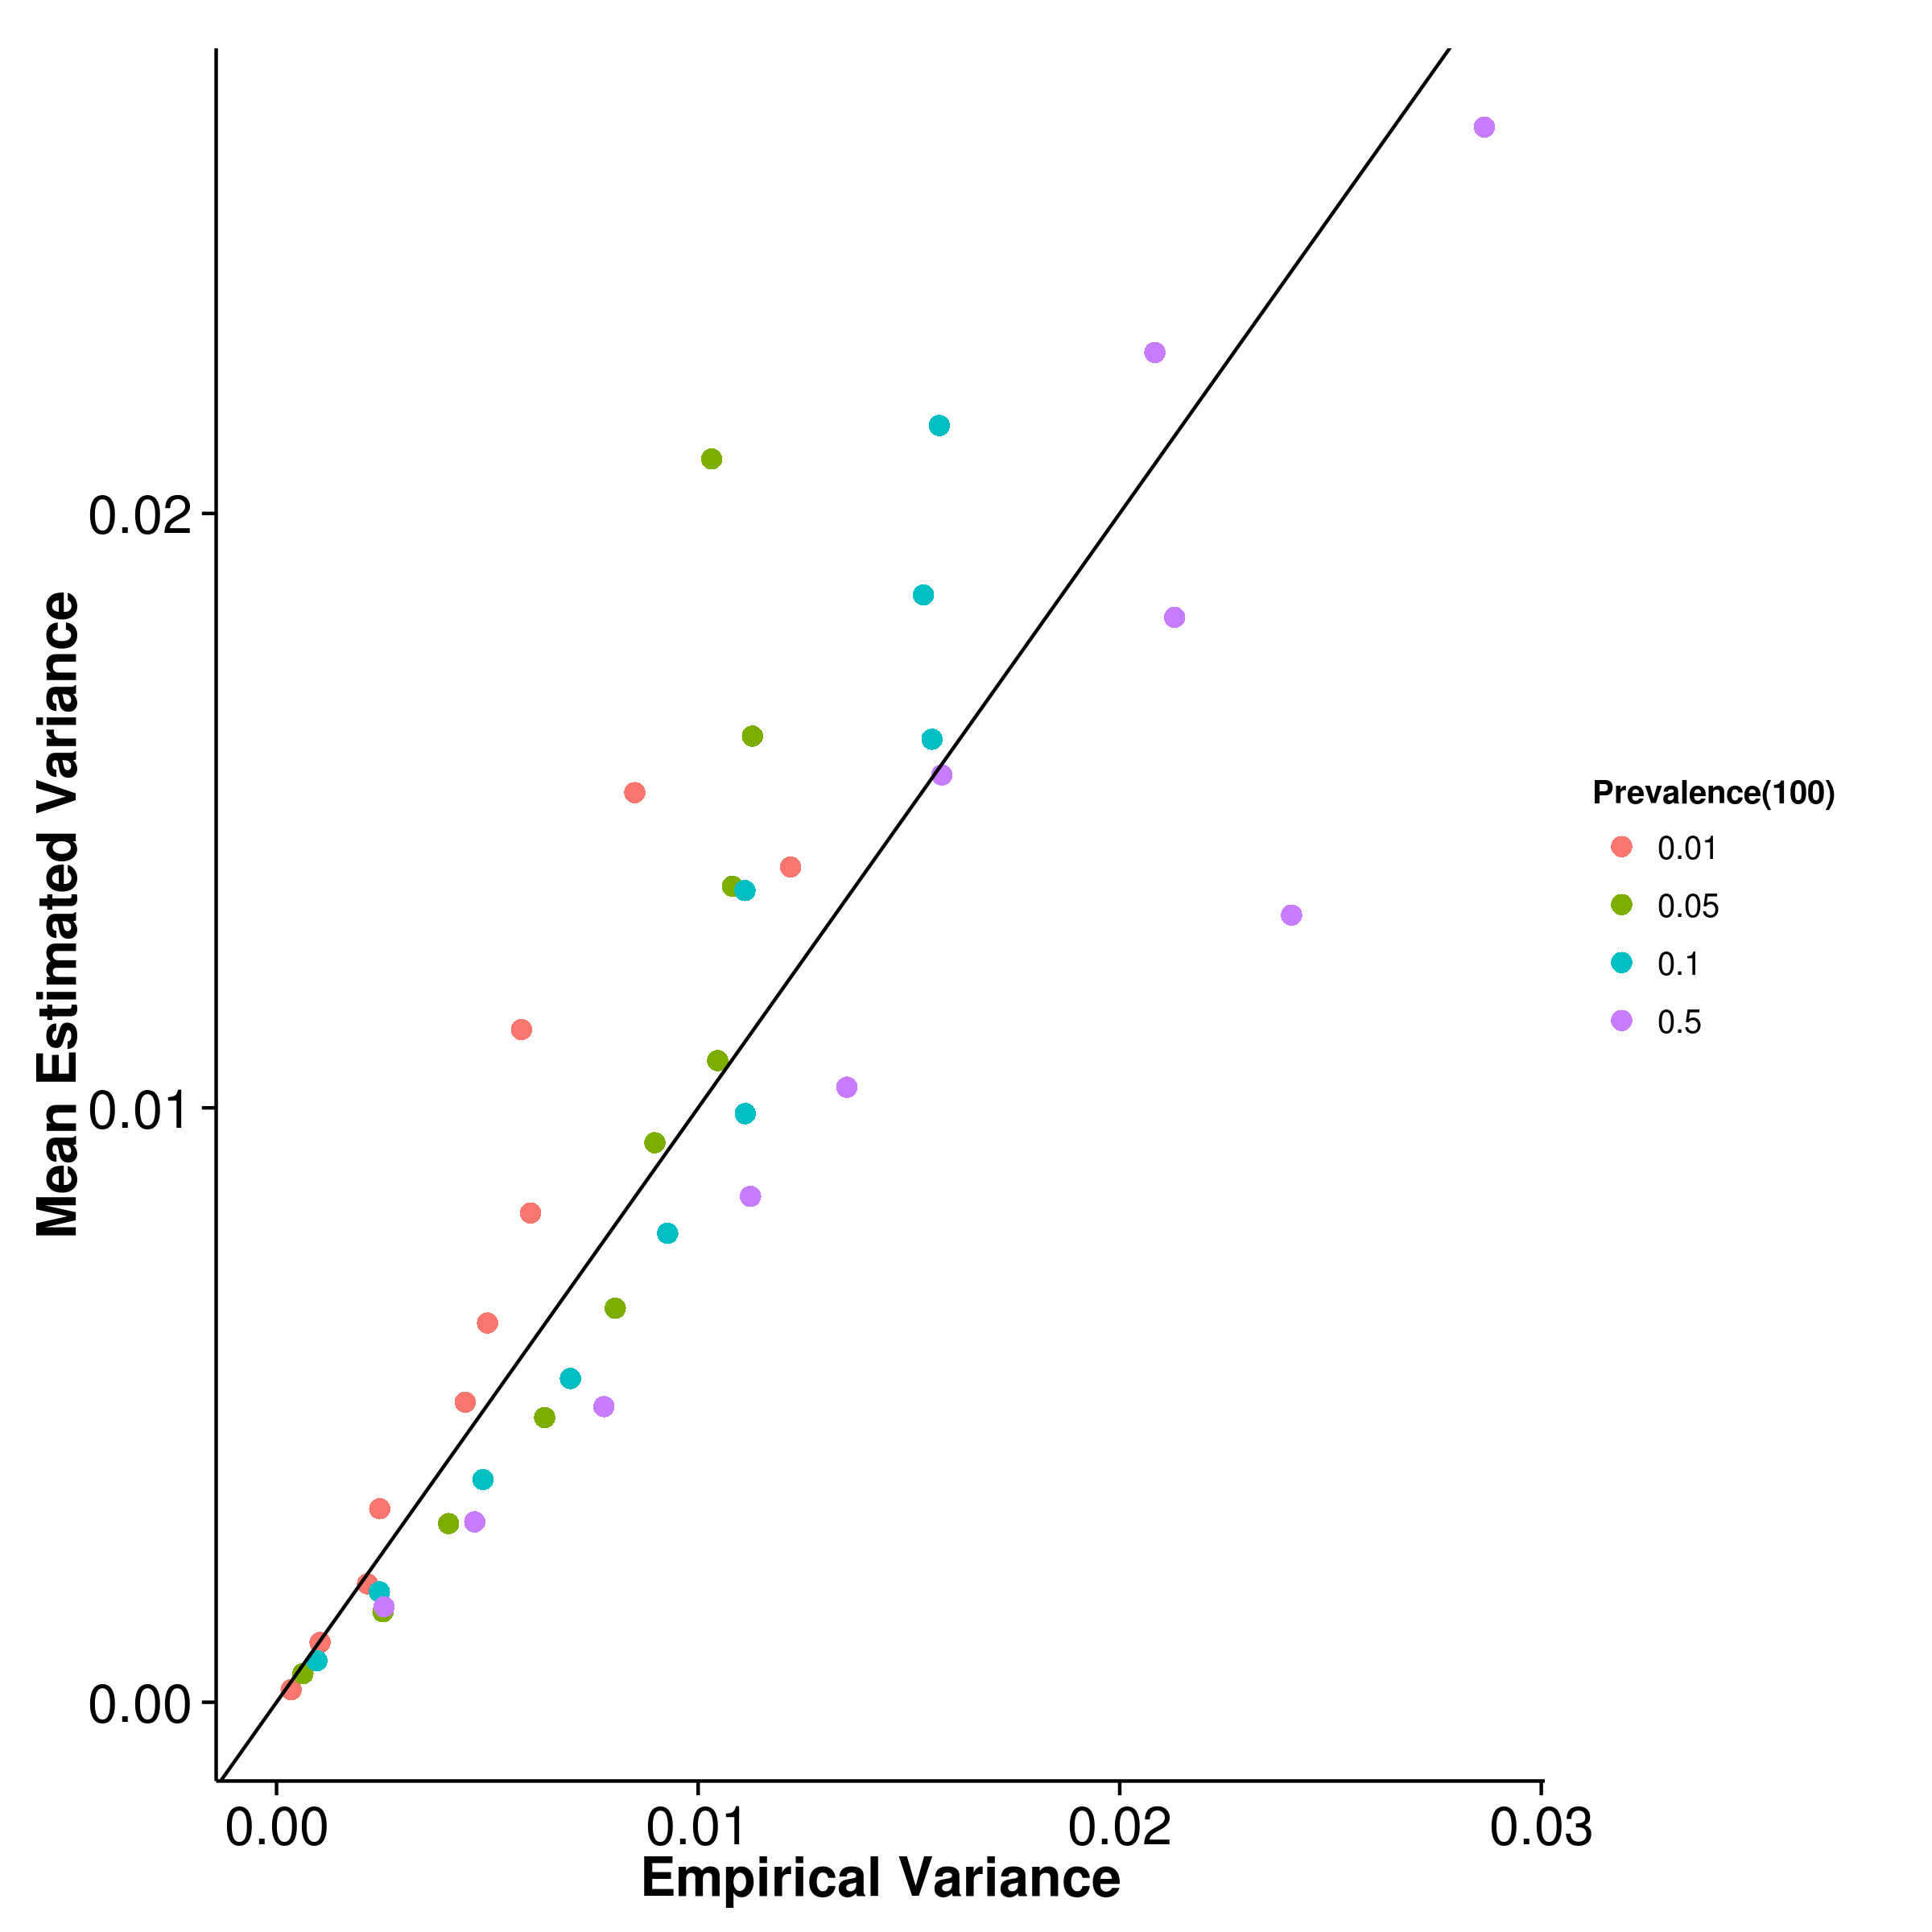
\includegraphics{figure/he_summary/cc_100c/ldscIn_CC_Rand_sdCom.png}}
				\label{fig:ldscInCCRandVarCom}
			}
			\caption[Estimation of Variance in Case Control Simulation (100 Causal)]
			{Estimated variance of results from case control simulation with random effect size simulation when compared to empirical variance when 100 causal \glspl{SNP} was simulated.
				Once again, \gls{shrek} underestimated its empirical variance and \gls{ldsc} with fixed intercept overestimates its empirical variance. 
				However, the magnitude of overestimation of \gls{ldsc} with fixed intercept decreased when compared to previous conditions. 
			} 
			\label{fig:CCRandVarCom}
		\end{figure}